\documentclass[FM,BP,EN,fonts]{tulthesis}

\usepackage{polyglossia}
\setdefaultlanguage{english}

\usepackage{makeidx}
\usepackage{enumitem}
\makeindex

\usepackage{xunicode}
\usepackage{xltxtra}
% potřebuji neproporcionální kurzívu, kterou Noto Sans Mono zatím nemá
\setmonofont{Roboto Mono}

\usepackage{setspace}
\setstretch{1.2}

\usepackage{parskip}
\usepackage{float} 
\usepackage{textcomp}

% příkazy specifické pro tento dokument
\newcommand{\argument}[1]{{\ttfamily\color{\tulcolor}#1}}
\newcommand{\argumentprom}[1]{\argument{\{\emph{#1}\}}}
\newcommand{\argumentindex}[1]{\argument{#1}\index{#1}}
\newcommand{\prostredi}[1]{\argumentindex{#1}}
\newcommand{\prikazneindex}[1]{\argument{\textbackslash #1}}
\newcommand{\prikaz}[1]{\prikazneindex{#1}\index{#1@\textbackslash #1}}
\newenvironment{myquote}{\begin{list}{}{\setlength\leftmargin\parindent}\item[]}{\end{list}}
\newenvironment{listing}{\begin{myquote}\color{\tulcolor}}{\end{myquote}}
\newcommand{\polozka}[1]{\item[#1]\mbox{}\\}

\clubpenalty=10000
\widowpenalty=10000
\sloppy

\tolerance=200
\emergencystretch=2em
\hyphenpenalty=10000
\hbadness=10000

% deklarace pro titulní stránku / title page declaration
\TULtitle{Sledování polohy v reálném čase s online výstupem}{Real-time location tracking with online output}
\TULauthor{Petr Boháč}

\TULprogramme{B0613A140005}{Informační technologie}{Information technology}
\TULbranch{B0613A140005AI-80}{Aplikovaná informatika}{Applied informatics}
\TULsupervisor{Ing. Jana Kolaja Ehlerová, Ph.D.}
\TULyear{2024}

% biblatex config
\usepackage[ 
    backend=biber
    ,style=iso-numeric
    ,autolang=other
    ,bibencoding=UTF8
    ,maxcitenames=2 %maximum v textu citovaných jmen
    ,maxbibnames=3 %maximum v seznamu vyjmenovaných autorů
    ]{biblatex}
\addbibresource{references.bib}

% Úprava iso-numeric.bbx v souladu s požadavky TUL hranaté závorky v číslovaném seznamu / Modification of iso-numeric.bbx in accordance with TUL requirements of square brackets in a numbered list
\DeclareFieldFormat{labelnumberwidth}{\mkbibbrackets{#1}}

% Formátování podle pokynů FZS, při využití stylu iso-authoryear, čárka mezi jmény a poslední jméno se spojkou a / special requirements of FZS TUL 
\DeclareDelimFormat{multinamedelim}{\addcomma\space}

\DeclareDelimFormat{finalnamedelim}{%
  \ifnumgreater{\value{liststop}}{2}{\finalandcomma}{}%
  \addspace\bibstring{and}\space}

\DeclareNameAlias{author}{family-given/given-family} 
%%%%%%%%%%%%%%%%%%%%%%%%%%

\usepackage{listings}
\usepackage[autostyle]{csquotes}
\urlstyle{same}

\newcommand{\aref}[1]{\hyperref[#1]{Appendix~\ref*{#1}}}

\usepackage{parskip}
\usepackage{hyperref}
\setlength{\parindent}{1em}
\setlength{\parskip}{0pt}

\newcommand{\source}[1]{\hfill Source: {#1}} %command definition for sources in figures

\begin{document}

\ThesisStart{zadani.pdf}
%\ThesisStart{male}

\begin{acknowledgement}
I would like to dedicate this section to all the people who have helped me to complete this thesis.

Firstly, a big thanks go to my thesis supervisor, Ing. Jana Kolaja Ehlerová, Ph.D., whose weekly consults have guided me in the right direction and eventually led to the successful completion of this thesis.

As this thesis is written in English and I am not a native English speaker, I've asked a handful of my close friends to review my work. Most notably, I am grateful to my dear friend Isaac Matthew Williams for providing the linguistic expertise. According to his words, \enquote{Even though I don’t know much about the topic at hand, I feel that I can grasp the material and follow along without getting lost}.

Finally, I'd like to express my gratitude to Caleb Andrews, MSc, from the University of Auckland, for offering invaluable technical feedback during the final stages of my thesis. Specifically his remarks regarding the authentication system.
\end{acknowledgement}

\begin{abstractEN}
This thesis explores the possibility of using the GNSS (Global Navigation Satellite System) to track everyday objects, most notably cars and other vehicles. 

A self-hosted solution has been developed, which utilizes the ESP32 microcontroller as the physical location data provider and a web application capable of receiving, processing, and presenting the mentioned data. The microcontroller uses a lightweight IoT communication protocol called MQTT, which transmits all the necessary data to the broker. The microcontroller has access to the Internet thanks to the integrated WiFi capabilities. 

The mentioned web application consists of a back-end server written in Java, handling all the business logic and exposing an API, which is then used by the front-end application built on top of the VueJS framework. All the data collected from one or more data sources is processed and stored in MongoDB, and the whole project is deployed in a containerized Docker environment.
\end{abstractEN}

\vspace{.5cm}

\begin{keywordsEN}
web application, navigation, MQTT, embedded development, wireless communication
\end{keywordsEN}

\vspace{2cm}

\begin{abstractCZ}
Tato práce zkoumá možnosti využití GNSS (Global Navigation Satellite System) ke sledování každodenních předmětů, zejména automobilů a jiných vozidel.

Bylo vyvinuto řešení s možností vlastního nasazení, které využívá mikrokontrolér ESP32 jako zprostředkovatele lokalizačních dat a webovou aplikaci schopnou přijímat, zpracovávat a prezentovat zmíněná data. Mikrokontrolér využívá nenáročný IoT komunikační protokol s názvem MQTT, který se stará o doručení dat na MQTT server. Mikrokontrolér má přístup k internetu díky integrovaným WiFi schopnostem.

Zmíněná webová aplikace se skládá z back-end serveru napsaného v Javě, který obsluhuje veškerou business logiku a zprostředkovává API, které poté využívá front-end aplikace postavená na frameworku VueJS. Všechna data shromážděná z jednoho nebo více datových zdrojů jsou zpracována a uložena v MongoDB a celý projekt je nasazen v kontejnerovém prostředí Docker.

\end{abstractCZ}

\vspace{.5cm}

\begin{keywordsCZ}
webová aplikace, navigate, MQTT, vývoj embedded systémů, bezdrátová komunikace
\end{keywordsCZ}

\clearpage

\tableofcontents

\clearpage

\listoffigures

\listoftables

\lstlistoflistings

\clearpage

\begin{abbrList}
\textbf{GPIO} & General-purpose input/output \\
\textbf{IoT} & Internet of Things \\
\textbf{WAN} & Wide Area Network \\
\textbf{QoL} & Quality of Life \\
\textbf{IO} & Input Output \\
\textbf{NMEA} & National Marine Electronics Association \\
\textbf{IDE} & Integrated Development Environment \\
\textbf{SSE} & Server-Sent Event \\
\end{abbrList}

\chapter*{Introduction}
\addcontentsline{toc}{chapter}{Introduction}
In today’s day and age, keeping track of our possessions is becoming increasingly important. From a security and safety standpoint, tracking objects like vehicles could be helpful in case of theft or, in an emergency, gaining location intel on a non-responding loved one. 

There are existing solutions on the market dealing with the issue at hand. Both in the open-source and commercial sphere. This project aims to develop a location-tracking solution, particularly for the \textbf{automotive industry}, featuring a full-stack application paired with a custom-built hardware package that can collect, process, and transmit location data wirelessly. The application will allow for managing collected data in an organized manner. Multiple users managed by one or more administrators may use the application concurrently and securely. Because the application allows for granular permission control, each user can be limited to a dedicated chunk of the collected data. Additionally, the need for extendibility is addressed through the inclusion of API keys and the selection of a flexible communication protocol. The entire application is securely deployed straightforwardly, ensuring both reliability and ease of use.

The initial chapter delves into a comprehensive analysis of the prevailing problem, examining existing alternatives while drawing comparisons among them. The discourse extends to GNSS's intricacies, encompassing theoretical frameworks, constellation configurations, and the role of Assisted GNSS (AGNSS) in location tracking. Furthermore, the chapter extensively explores diverse platforms and communication methodologies that may be used for the development of the hardware package.

The second chapter describes the construction of the hardware solution alongside the development of the embedded firmware. This chapter covers everything from the physical wiring to the software side of things.

In the following chapter, \autoref{chap:application}, the whole development process of the application is covered thoroughly. As the application is made up of two distinct components, each one is allocated its dedicated section. These key parts are segregated due to the disparate nature of technologies employed, representing two distinct realms within the project.

In \autoref{chap:results}, results are examined and discussed. Various implications regarding storage, sampling, and more are also touched upon. Additionally, the cost of the whole project is broken down.

Finally, in \autoref{chap:integration}, the discussion revolves around integration possibilities. As mentioned earlier, the solution was developed with scalability in mind. Several design choices were carefully made to facilitate seamless integration, maximizing the system's adaptability.

\chapter{Problem analysis}
\label{chap:problem-analysis}
The following chapter is dedicated to analyzing the problem at hand. As this is not the first project of its kind, a couple of existing solutions will be covered and compared. Furthermore, topics like collecting positional data and getting it where it's needed will also be touched upon as well.

\section{Available solutions}
In this section, a few alternatives, both open-source and commercial, will be discussed and later briefly compared to this project.

\subsection{Traccar}
The most popular modern alternative used in the present day is \textbf{Traccar}. It is a leading open-source GPS tracking system that supports over 200 GPS protocols and more than 2000 models of GPS tracking devices. Traccar offers exceptional performance, stability, and a modern web interface optimized for both desktop and mobile devices. It provides a paid cloud-based deployment. Due to its open-source nature, it can also be self-hosted \cite{traccar}.

\subsection{OpenGTS}
Another notable open-source project of a similar nature is \textbf{OpenGTS}. It was the first open-source project designed specifically to provide web-based GPS tracking services for a "fleet" of vehicles. The initial tutorial and guide for OpenGTS dates back to 2010. Despite its inception date, OpenGTS remains relevant today, with recent version updates as recent as 2020. The continuous utilization of OpenGTS in various countries and industries indicates its ongoing presence and relevance in the GPS tracking technology landscape \cite{opengts}.


\subsection{GPS Dozor}
Regarding product choices, regardless of the field, the commercial sphere often offers a plethora of choices and a wide range of features compared to free, open-source solutions. This abundance stems from companies' resources and investments in developing proprietary solutions tailored to specific needs.

In the Czech market, one prevalent option is \textbf{GPS Dozor}. Renowned for its reliability and comprehensive feature set, GPS Dozor caters to various industries, offering functionalities such as real-time tracking, route optimization, and comprehensive reporting tools. A massive selling point of GPS Dozor is its powerful, organized dashboard that users can use to manage their entire fleets of vehicles. Its popularity underscores its effectiveness in meeting the needs of businesses operating in the region.


\subsection{Track Your Truck}
Outside of Czechia, \textbf{Track Your Truck} emerges as a prominent player in the commercial GPS tracking sphere. With a strong presence in the United States and beyond, Track Your Truck provides customizable solutions tailored to diverse business requirements. Its offerings include advanced fleet management features, integration capabilities with other business systems, and specialized solutions for specific industries such as transportation, construction, and logistics.

Both GPS Dozor and Track Your Truck exemplify the diversity and innovation in the commercial GPS tracking market, offering businesses and individuals a wide array of options based on their specific needs and preferences.

\section{Obtaining positional data}
The key function of a data source is collecting positional data, among other things. This section will focus on the issue of getting that positional data reliably. Nowadays, the standard way to determine one's coordinates is GNSS.

\subsection{Theory behind Global Navigation Satellite Systems}
The need to determine one's position on Earth dates all the way back to the mid-20th century during the Cold War era. The United States Navy, in the 1960s, initiated the first satellite navigation system dubbed Transit. Its primary use was to provide the U.S. Navy with accurate location information to be used by their Polaris ballistic missile submarines. Other use cases included surveying and providing the Navy's surface ships with positional intel. In the late 1970s, the U.S. began developing the Navstar Global Positioning System, now known as GPS, to overcome some of the Transit's limitations. GPS, unlike Transit, was designed to offer highly accurate global coverage that is available to both the military and civilians.

GNSS (Global Navigation Satellite System) is a general term for any satellite constellation\footnote{A satellite constellation is a group of satellites orbiting the Earth and working together as one system} \cite{esa}. Currently, multiple GNSS constellations are orbiting the Earth, each of which is briefly described in \autoref{subsec:constellations}. Everyday devices like smartphones, watches, etc., usually come equipped with GNSS receivers out of the box. A GNSS receiver ("receiver") is generally a hardware device which is able to pick up the signals transmitted by satellites, process them, and provide the user with positional data. 

Contrary to popular belief, GNSS is a one-way communication system, meaning data goes only one way; no back-and-forth communication is happening. A GNSS satellite is nothing more than an incredibly precise clock; an atomic clock in fact. The precision of these clocks is a crucial part of a GNSS, as it heavily relies on measuring the time of arrival of radio signals. Thus, each GNSS system has its own time reference from which everything is synchronized. Satellites broadcast signals, that, among other things, contain the precise current timestamp and location of that satellite. When a receiver is first turned on, it listens for GNSS signals. The first connected satellite transmits the \textit{almanac}, which gives the receiver a general idea of where all the satellites in the constellation are. To determine the precise location, more than one satellite is needed. The process of calculating the position is called \textit{trilateration}, not to be confused with triangulation. The name suggests that 3 points, or satellites in the context of GNSS, are needed to get a position fix\footnote{A position fix is the successful result of GNSS positioning, indicating the receiver's location with a given accuracy}. Even though three satellites are the theoretical minimum for obtaining a fix, receivers generally require at least 4 satellites. The additional satellite allows for greater precision, and is taking the positioning from 2D to 3D, providing us with altitude. In general, the more satellites feeding the receiver with data, the greater the precision. With support from other systems, sub-centimeter geolocation precision is possible in today's world.

\subsection{GNSS constellations}
\label{subsec:constellations}
The previous section mentioned the presence of multiple GNSS constellations. Today, there are \textbf{four} core global active GNSS constellations

\begin{itemize}
    \item \textbf{GPS} (31 satellites) \cite{gps}
        \begin{itemize}
            \item First launch year: 1978
            \item World's most utilized satellite system developed and maintained by the U.S. Department of Defense
            \item Guaranteed 95\% availability of at least 24 satellites (for redundancy purposes, up to 32 satellites are in use today)
        \end{itemize}
    \item \textbf{GLONASS} (24 satellites) \cite{glonass}
        \begin{itemize}
            \item First launch year: 1982
            \item Formerly Soviet, now Russian space-based satellite 
            navigation system
            \item Full global coverage since 1995
        \end{itemize}
    \item \textbf{BeiDou} (44 satellites) \cite{beidou}
        \begin{itemize}
            \item First launch year: 2000
            \item Started as an Asia-Pacific local network. Owned and operated by the China National Space Administration
            \item Global coverage was reached in 2018
        \end{itemize}
    \item \textbf{Galileo} (23 satellites) \cite{galileo}
        \begin{itemize}
            \item First launch year: 2011
            \item Created by the EU through ESA (European Space Agency), operated by the EUSPA, headquartered in Prague, Czechia
        \end{itemize}
\end{itemize}

There are two more regional navigation satellite systems worth mentioning.

\textbf{NavIC} is an autonomous regional satellite navigation system covering the region of India. It is operated by the ISRO (Indian Space Research Organisation). Since its first launch in 2013, 10 total launches have been completed, deploying seven satellites in the process \cite{navic}.

The second system is the \textbf{QZSS} (Quasi-Zenith Satellite System), a four-satellite regional system developed by the Japanese government. It was first launched in 2010 to enhance the United States-operated GPS in the Asia-Oceania region \cite{qzss}.

\subsection{Assisted GNSS}
As stated, GNSS uses satellites, which transmit information using radio signals. These radio signals aren't very strong \cite{gnss-accuracy}.

Receivers usually have three start modes - cold, warm, and hot.

When a receiver has been powered off for a long time, usually over two hours, it almost certainly lacks or has outdated almanac and ephemeris data. In this case, after the receiver powers up, it must obtain the almanac from the first satellite it connects to, followed by ephemeris data from at least four satellites to acquire a 3D fix. All of this data gathering, together with calculating the coordinates, takes a considerable amount of time (the almanac alone takes approx. 12.5 minutes to transmit); therefore, this is referred to as a \textbf{cold start}.

If the receiver has a valid up-to-date almanac and thus roughly knows where the satellites are in orbit, it must only acquire ephemeris from each satellite before it can start calculating the coordinates. This is a so-called \textbf{warm start}.

A \textbf{hot start} happens when the receiver has both a valid, up-to-date almanac and ephemeris in its memory. In this case, it has everything it needs and can start calculating a precise location \cite{gnss-start-modes}.

Due to the strength of signals transmitted by satellites, near-perfect conditions are required for GNSS to function optimally and reliably. Sky obstructions like big buildings or going underground might very well cause the loss of a positional fix.
In fact, most smartphones don't directly use GNSS at all; they all use assisted GNSS, where the position is calculated with the help of cellular towers with known coordinates acting as positional references.

\section{Available platforms}
\label{sec:platforms}
In the process of constructing a hardware solution of any kind, an engineer's initial and foremost responsibility lies in selecting the appropriate platform. Each project possesses unique requirements, with certain factors holding greater significance than others. 

While Arduino, Espressif, and Raspberry Pi dominate the microcontroller market, it's noteworthy that smaller players, such as Adafruit and Teensy, have also made significant strides, contributing their unique offerings to the hardware ecosystem. For simplicity's sake, the following discussion and comparison will focus solely on the three main contenders in the microcontroller space.

This project has a few specific needs that dictate the platform selection. Firstly, the device must operate with minimal power consumption to ensure prolonged battery life if used in conjunction with a small battery. 

Secondly, it requires seamless connectivity to transmit GPS data efficiently, whether for real-time tracking or data logging purposes. 

Additionally, compact size is essential to facilitate a sleek and portable design for the GNSS tracker device. 

Furthermore, the microcontroller must possess sufficient processing power to handle real-time data processing tasks efficiently. 

Finally, cost-effectiveness is a crucial factor, especially considering the circumstances and the fact that this project is not backed by a larger entity willing to take the cost out of the equation.

\subsection{Arduino}
When there is a need for more complex logic that involves programming in electronics, novice tinkerers often reach for an \textbf{Arduino} board of some sort, e.g. an Arduino UNO as seen in \autoref{fig:arduino}. Arduino is an open-source platform spanning both the physical (hardware) and the software components. Arduino is widely used amongst hobbyists for its simplicity and versatility. A vast community built around Arduino is populating the Internet with countless tutorials, guides, and articles, significantly flattening the learning curve. Arduino even has its own simple IDE, which makes it really simple to develop and deploy code to the microcontroller \cite{what-is-arduino}.

\begin{figure}[H]
    \centering
    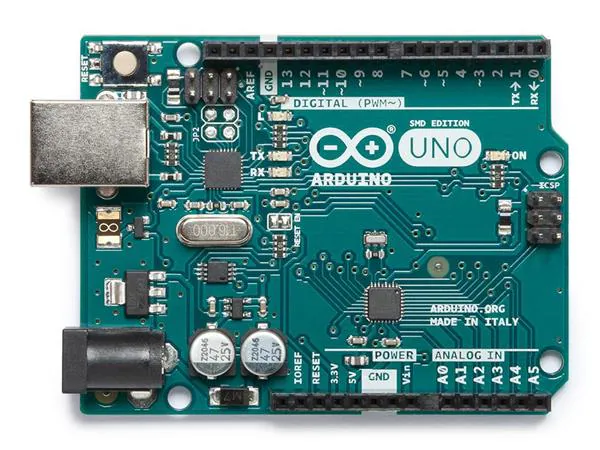
\includegraphics[scale=.3]{media/arduino.png}
    \caption{Arduino UNO}
    \textit{Source:} https://cz.mouser.com
    \label{fig:arduino}
\end{figure}

\subsection{Raspberry Pi}
Unlike Arduino, which typically caters to the lower end of the spectrum in terms of processing power, price, and overall capabilities, \textbf{Raspberry Pi} occupies the higher end. While Arduino boards are renowned for their simplicity, cost-effectiveness, and suitability for basic to moderately complex projects, Raspberry Pi offers significantly more processing power, versatility, and features. In January 2021, the Raspberry Pi Foundation came out with its first microcontroller, the \textit{Raspberry Pi Pico} (see \autoref{fig:raspberry}), based upon a single chip, the RP2040.

\begin{figure}[h]
    \centering
    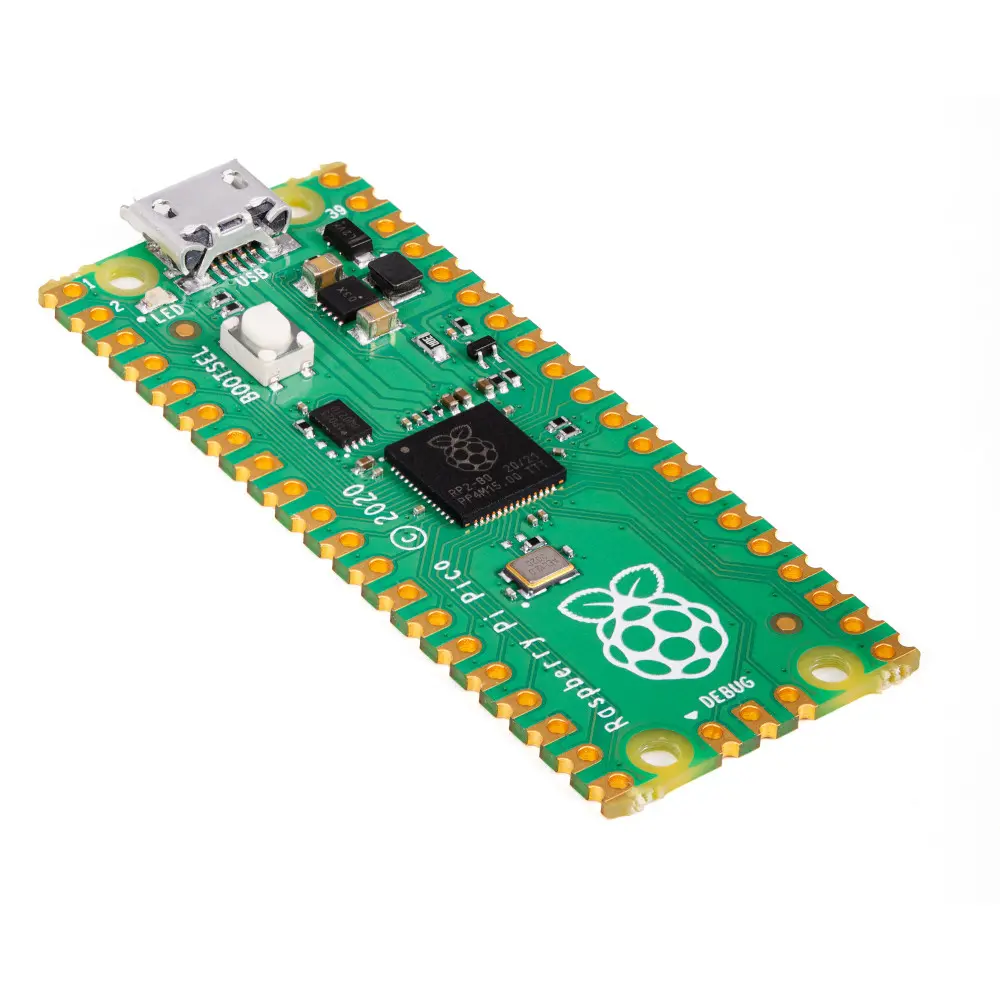
\includegraphics[scale=.2]{media/rpipicow.png}
    \caption{Raspberry Pi Pico }
    \textit{Source:} https://rpishop.cz
    \label{fig:raspberry}
\end{figure}

\subsection{Espressif}

If neither Arduino nor Raspberry Pi meets a project's needs, there is another viable option worth considering: \textbf{Espressif Systems}. Among its standout offerings are the ESP8266 and ESP32 (as seen in \autoref{fig:esp32}, utilized in a development board), popular choices for hobbyists and large corporations alike. 

An excellent example of IoT products based on the ESP chips are those from Shelly. Their range includes smart plugs, energy meters, and more. T

he ESP32 is a successor to the ESP8266, equipped with a Dual-Core 32-bit LX6 Microprocessor with a clock frequency of up to 240 MHz, 520 KB of SRAM and 448 KB of ROM. It also has 34 Programmable GPIO pins, allowing for a vast amount of external switches, LEDs, and sensors, which is a cruicial requirement for this project.

\begin{figure}[h]
    \centering
    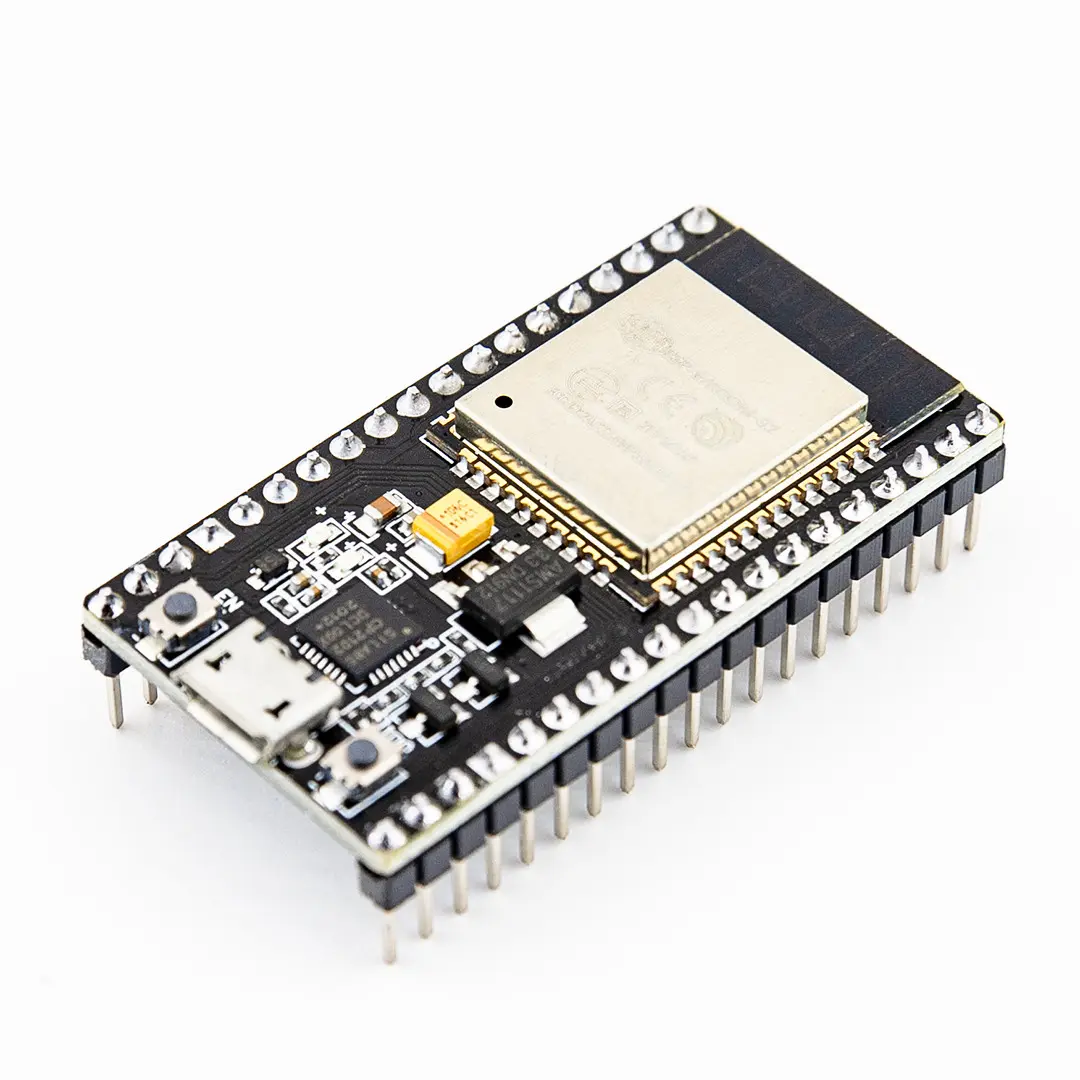
\includegraphics[scale=.2]{media/esp32.png}
    \caption{ESP32 development board}
    \textit{Source:} https://rpishop.cz
    \label{fig:esp32}
\end{figure}

\subsection{Conclusion}

Several key requirements must be considered when selecting the correct microcontroller for this project. Given the complexity of the firmware, which would incorporate multiple libraries to support intricate logic, as well as the necessity for a management web application to run directly on the microcontroller for configuration and debugging purposes, resource utilization became a critical factor. 

The chosen microcontroller needed to offer sufficient CPU power to handle the computational demands of the firmware and web application. Moreover, it was essential to ensure an adequate amount of RAM and ROM to accommodate the simultaneous operation of these features without compromising performance. 

In addition to the processing power and memory requirements, WiFi connectivity was identified as a non-negotiable key feature for this project.

After thorough research, testing multiple different options, and careful consideration of their strengths and weaknesses, the ESP32 microcontroller emerged as the optimal choice for this project. Specifically, the Espressif development board \textbf{ESP-WROOM-32 DEVKIT V1} was selected to fulfill the project's requirements.


\section{Methods of communication}
\label{sec:comm-methods}
A crucial part is figuring out how to connect the hardware client to the back-end server. The possible solution set highly depends on where the server is physically located. Choosing the right communication technology really depends on the project's specific needs. In this section, various wireless communication technologies will be discussed and compared.

\subsection{Mesh networks}
Some technologies are ideal for situations where the device is deployed permanently and never moved. For these cases, mesh networks are usually the best option. In the world of IoT, two\footnote{Although Zigbee and Z-Wave dominate the sphere, several new protocols have been on the rise in the past few years, most notably Thread and Matter.} stand out the most - the \textbf{Zigbee} and \textbf{Z-Wave} protocols. Both of these protocols were developed to tackle similar issues but have some differences. Zigbee is a low-power wireless mesh network standard targeted at battery-powered devices in wireless control and monitoring applications. Right after WiFi, it's the most common way for smart devices to communicate. Its implementation in products is an easy and cheap way to broaden the product's flexibility \cite{zigbee}. Zigbee operates at the same frequency as WiFi - 2.4GHz.

Z-Wave is an alternative to Zigbee aimed at the same applications. It operates at a much lower frequency (800-900 MHz as opposed to Zigbee, which, alongside WiFi, operates in the 2.4 GHz range) \cite{zwave}. The major selling point of Z-Wave is its rigorous certification protocol. All products using Z-Wave have to undergo a special certification process, which guarantees a smooth deployment and reliable operation \cite{zwave-certification}. This adds time and complexity to the product development, increasing the product's price. That is why nearly all Z-Wave products tend to be more expensive than their Zigbee counterparts.

In summary, IoT protocols such as Zigbee and Z-Wave are good low-power communication technologies most smart home products use. They are mostly used to bridge the gap between the devices and a smart home hub, usually connected and integrated over TCP/IP to the rest of the network. This project requires direct access to the Internet to be able to communicate with the server. In this case, using Zigbee or Z-Wave would add an unnecessary middleman. Therefore, these communication technologies are also \textbf{not applicable} in this case.

\subsection{Short range}
Bluetooth is a very simple wireless technology standard mainly aimed at short-range communication. Nowadays, it's well supported for a wide range of devices. The usable range of Bluetooth depends on multiple factors, such as \cite{bluetooth-range}:
\begin{itemize}
    \item Radio Spectrum
    \item Receiver Sensitivity
    \item Transmission Power
\end{itemize}

Bluetooth is usually utilized to configure devices. Because it requires the two participating devices to be in proximity to each other. For instance, configuring solar inverters, smart power plugs, etc.

This technology may be useful when the server - in the context of a car - sits in the cabin with the data source. As this would be a very specific and limiting case, Bluetooth \textbf{does not} meet all the needs for it to be used as the main way of communication between the data source and the back-end server.

\subsection{Long range}
When researching long-range communication technologies, the first one to come to mind is LoRa (short for "long-range"). It aims to address the challenge posed by the growing distances over which data needs to be wirelessly transmitted in the era of IoT. While existing technologies like WiFi and cellular excel at moderate distances and meet high bandwidth demands, they fall short for longer transmissions (as depicted in \autoref{fig:lora-wifi-cellular-comparison}). LoRa devices and networks, such as \textbf{LoRaWAN}, enable smart IoT applications addressing challenges in energy management, natural resource reduction, pollution control, infrastructure efficiency, disaster prevention, and many more \cite{what-is-lora}. 

\begin{figure}[H]
    \centering
    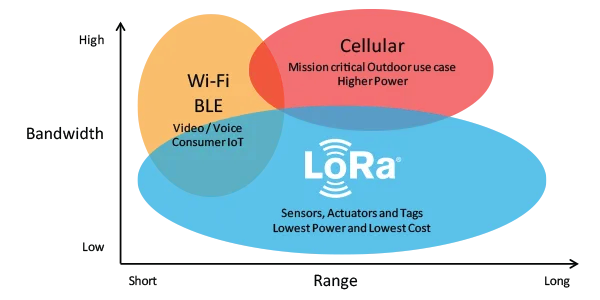
\includegraphics[scale=.7]{media/lora-bandwidth-vs-range.png}
    \caption{Bandwidth and range comparison}
    \textit{Source:} https://www.thethingsnetwork.org/docs/lorawan/what-is-lorawan/
    \label{fig:lora-wifi-cellular-comparison}
\end{figure}

LoRaWAN is a standard for interoperability managed by the LoRa Alliance, a non-profit technology alliance, and is recognized as an LPWAN standard by the International Telecommunication Union (ITU). Devices utilizing LoRa for data transmission usually have an outstanding battery life due to LoRa's nature. Some reported lasting as long as ten years on a single coin cell battery. LoRaWAN operates through gateways, forming networks that cover vast geographical regions. The range of these gateways varies based on their placement and local environment. While wireless transmissions often face interference, LoRaWAN offers impressive capabilities. In rural settings, a gateway can extend its reach up to 3 kilometers, but in more open areas, distances exceeding 10 kilometers are achievable. Moreover, LoRaWAN has the unique ability to locate end devices through triangulation, eliminating the need for GPS \cite{what-is-lorawan}.

LoRaWAN is a great choice for applications requiring communication across large geographical areas, but the coverage is not quite where it needs to be for this project. This is where cellular comes in.

\textbf{Cellular communication} is built upon terrestrial cellular towers (as shown in \autoref{fig:cell-tower}); hence the name. Cellular towers can cover anywhere from 5 to 80 square kilometers, so they are strategically placed to cover as much area as possible. Cellular equipment is often conveniently installed on existing buildings or structures, or an actual tower is constructed for that exact purpose. Multiple mobile network operators almost always share a "cell site" so that as many people as possible have connectivity regardless of their carrier.

\begin{figure}[H]
    \centering
    \includegraphics[scale=.25]{media/cell-tower.jpg}
    \caption{Top of a cellular tower}
    \textit{Source:} https://commons.wikimedia.org/wiki/File:CellTowerRichmondHill.jpg
    \label{fig:cell-tower}
\end{figure}

As previously stated, the function of a cellular-based communication device relies on the proximity of cell towers. Roughly one-third of the land is covered by cell towers \cite{mobile-network-coverage}. Cell towers are installed on demand; more are installed in areas with higher population density. The difficulty of implementing cellular communication into a project depends on multiple factors. Some microcontrollers are specifically designed for off-grid applications. Therefore, they might come pre-equipped with cellular radio and a SIM card slot. As this might not be the case with the microcontroller chosen for this project, it's important to consider the added complexity and cost that implementing cellular communication would introduce.

\subsection{WiFi}
Defined by the IEEE 802.11 family of standards, \textbf{WiFi} serves as a wireless transmission medium within the confines of a communication channel. Nevertheless, it does not inherently provide direct internet connectivity. Instead, it facilitates communication with another device, typically a router, which is then linked to a Wide Area Network (WAN). This WAN connection can be established through various means, such as the previously mentioned cellular networks, wireless bridges, wired connections, or optical fibers \cite{what-is-wifi}. When evaluating WiFi for a project, it's essential to consider both its advantages and disadvantages. On the positive side, WiFi boasts widespread adoption and accessibility, making it easy and relatively inexpensive to implement. Many microcontrollers come equipped with integrated WiFi capabilities, streamlining the hardware setup process. Additionally, WiFi delivers decent data transfer speeds and can accommodate moderate to high bandwidth requirements, rendering it suitable for various applications. Nevertheless, there are drawbacks to take into account. WiFi tends to consume more power than other wireless technologies, posing a concern for battery-powered devices or those necessitating low power consumption.

Therefore, after careful consideration of its pros and cons, WiFi was chosen as the \textbf{preferred communication medium} for this project due to its ease of use, cost-effectiveness, and suitability for meeting the project's requirements.


\section{Data delivery}
\label{sec:data-delivery}
As the issue of connecting data sources to the Internet has already been addressed and resolved in \autoref{sec:comm-methods}, now comes the issue of delivering the collected data to the back-end server. There are many ways to exchange data between services: gPRC, STOMP, MQTT, or simple HTTP requests, to name a few. For the purposes of this project, only the last two methods will be taken into consideration.

Using HTTP for data exchange is a simple and readily used method. Clients needing data exchange can issue an HTTP request (a POST request would make the most sense here) to a web server running on the other system, which extracts and processes the data from the request. In this case, data sources send the collected data to the server very frequently. Thus, most of the communication the data sources participate in consists of many small data bundles. HTTP requests are a bit costly compared to some of the alternatives. HTTP used to create a new TCP connection for every request. Since HTTP 1.1, there are some TCP connection pooling capabilities, but the overhead is still present due to other factors (authentication, for instance). Data sources might be working with a limited Internet connection, meaning conservative and efficient approaches to data transmission are required. In summary, HTTP request-based data exchange is a valid approach, but a better one is needed for this use case.

\textbf{MQTT} (Message Queuing Telemetry Transport) is a communication protocol based on a publish/subscribe model with features specifically targeted at IoT solutions. MQTT aims to minimize the data overhead of each MQTT packet. It has many advantages of the previously mentioned HTTP request-based approach, including \cite{mqtt-v-http}:
\begin{itemize}
    \item Uses a single long-lived TCP connection
    \item As opposed to HTTP, which was designed to serve documents on the Internet, MQTT was specifically designed for IoT
    \item Binary message payloads instead of text-based HTTP payloads
    \item other useful features for IoT applications
\end{itemize}



\chapter{Hardware solution implementation}
The first half of this thesis is expected to produce a hardware solution that is able to collect positional data reliably and securely transmit them back to the server. 

The main hardware package ("Data source") is wired up on a breadboard, which allows for rapid development and easy reconfiguration at any point. As was established in \autoref{sec:platforms}, an ESP32 was selected as the microcontroller of choice.

The different ways to install and deliver power to the device are out of the scope of this thesis.

\section{Construction}
When developing a hardware solution of any kind, there are usually two stages to the whole process. In the development stage, everything is thoroughly tested and finalized to the developer's satisfaction. At this point, the product is usually pieced together on a breadboard (shown in \autoref{fig:breadboard}). The individual components are connected together, either by placing them strategically, taking advantage of the breadboard's inner conductors, or by using jumper cables (most commonly DuPont-style wires).

\begin{figure}[ht]
    \centering
    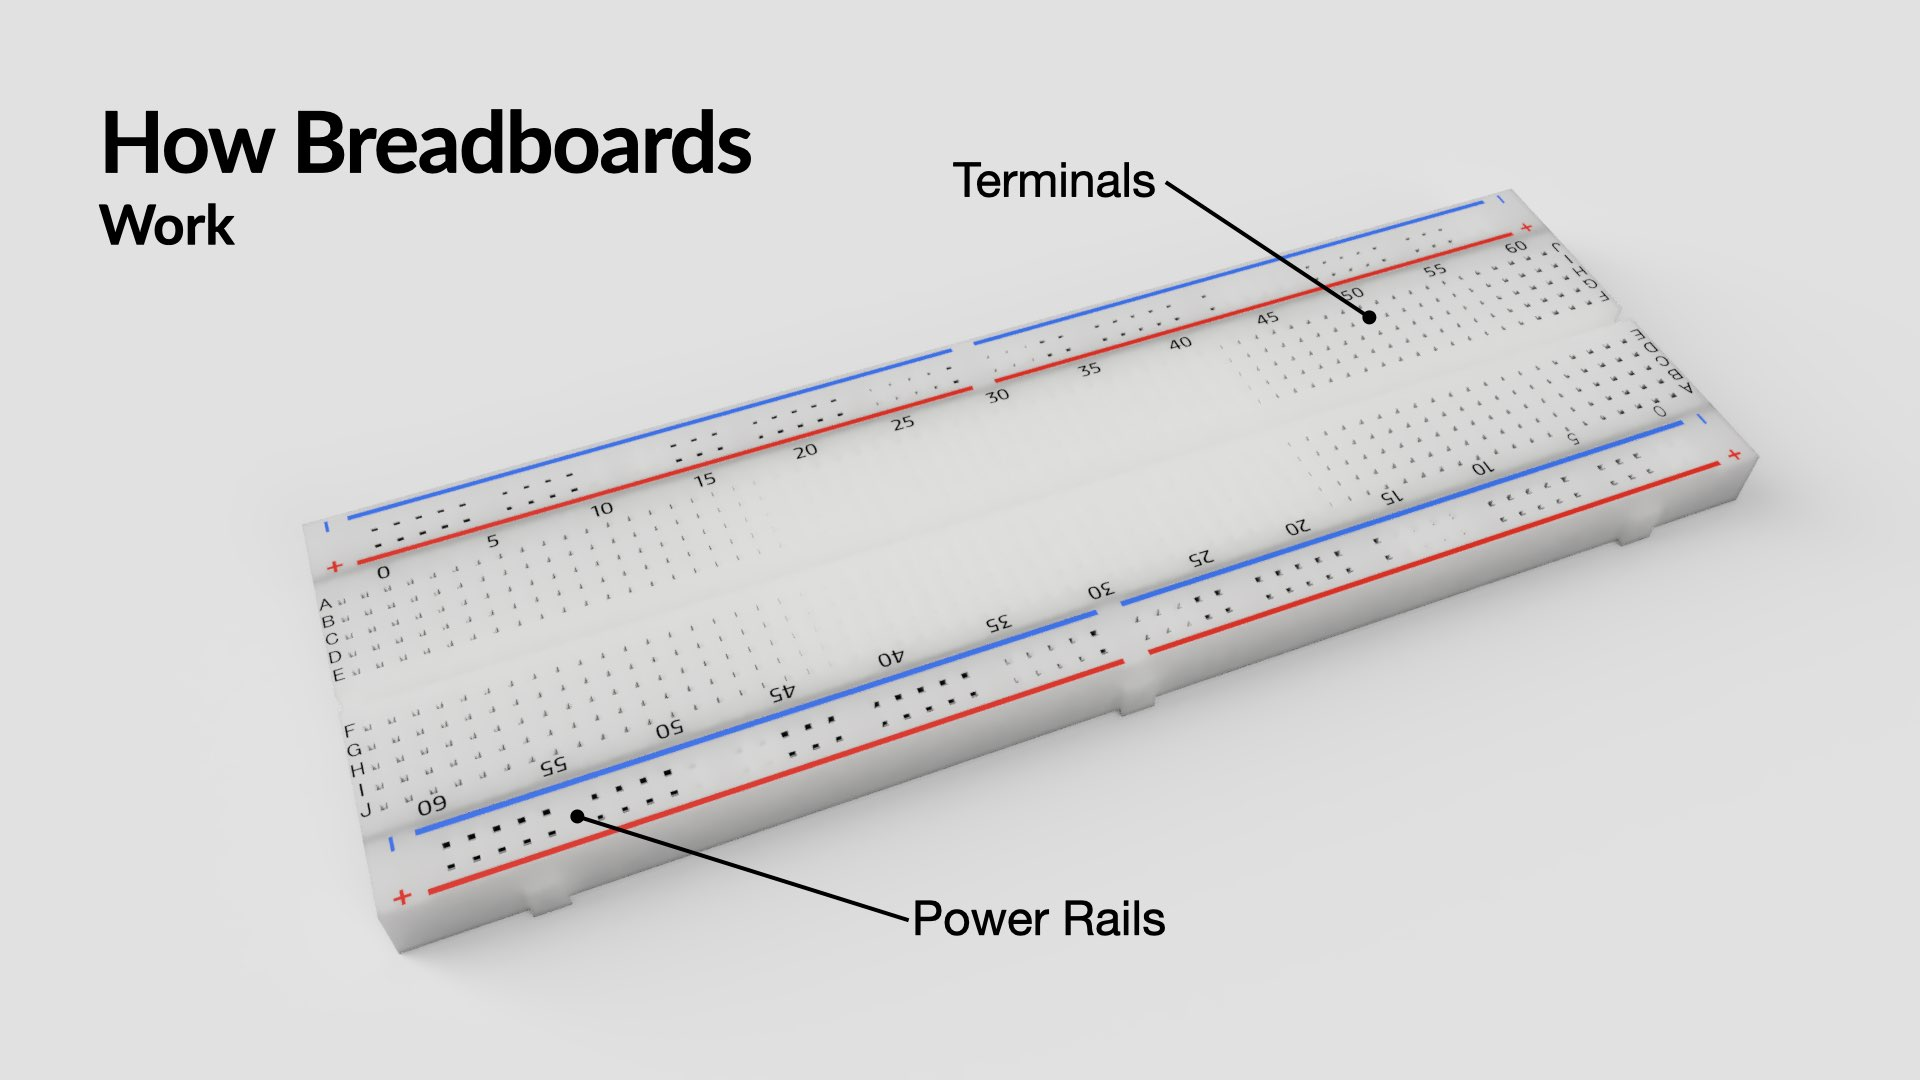
\includegraphics[scale=.2]{media/breadboard.jpg}
    \caption{A development breadboard}
    \textit{Source:} https://www.kevsrobots.com/resources/how\_it\_works/breadboards.html
    \label{fig:breadboard}
\end{figure}

The product design is finalized in the latter stage - the production stage. If needed by the circumstances of the product's usage, an enclosure might be designed and produced. The most common manufacturing process for new products nowadays is 3D printing. Injection molding is also a popular process for a more professional-looking final product, although it comes at a higher cost.

\subsection{Wiring diagram}
Part of any hardware realization or product is the wiring diagram. The wiring diagram is a crucial blueprint within any hardware realization or product development process, facilitating seamless construction and ensuring operational success. Comprised of standardized components meticulously labeled for clarity, this diagram is a guiding map for technicians and engineers, enabling them to comprehend and implement intricate electrical connections accurately. By integrating these standardized elements, the diagram simplifies the construction process and enhances compatibility and interoperability, streamlining overall operations and fostering efficiency. This visual representation forms an indispensable tool, bridging the gap between conceptual design and tangible implementation, ultimately contributing to realizing reliable and functional hardware solutions. The wiring diagram for this project (as seen in \autoref{fig:diagram}) was drawn using a designer tool called Circuit Diagram Online.

\begin{figure}[p]
    \centering
    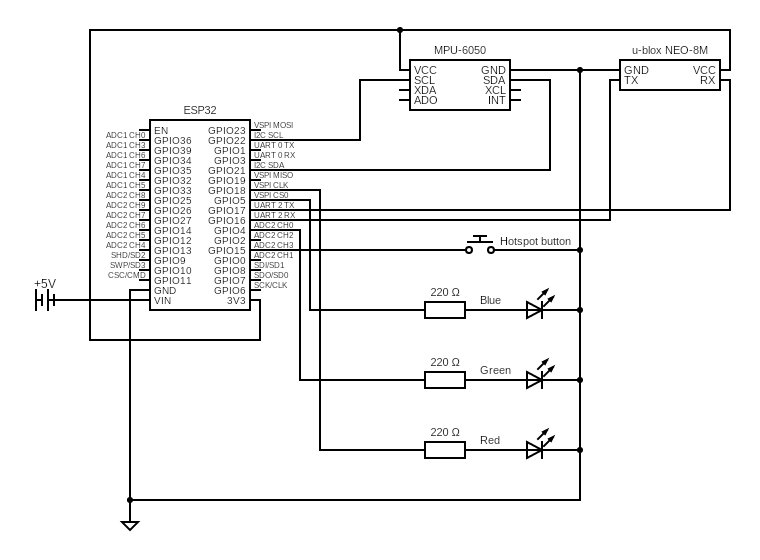
\includegraphics[scale=.6]{media/circuit.png}
    \caption{The wiring diagram of the hardware solution}
    \label{fig:diagram}
\end{figure}

\newpage

\section{Physical controls}
\label{sec:physical-data-source-controls}
All of the data source configuration is done using the web application served by the ESP. It can also be used to interact with the data source at runtime, but this is not optimal, as it does not have a straightforward user experience; the user needs to use a device with a browser and must make sure they're connected to the data source. For that reason, there is a need for physical controls that can make changes and interact with the data source at runtime.

When the WiFi hotspot ("hotspot") is turned on and anyone can connect to it (it is not secured with a password). The web application served by the ESP requires no authentication either. Therefore, the less time the hotspot is being broadcast, the better. A hotspot toggle button was implemented to counteract this issue. When the data source is connected to power, it initially starts with the hotspot being turned off; the user must press the button to turn the hotspot on to configure it. After all necessary configurations have been made, it is encouraged to turn the hotspot off.

\section{Visual indications}
Having a good looking intuitive dashboard with all the relevant information at a quick glance is nice, but when it comes to hardware solutions, it is expected to have a way for the user to roughly tell what is currently happening. A potential solution for this problem could be a small integrated screen displaying information. Seven-segment displays would also be a sufficient solution if the information were just a number. The most straightforward kind of indicators are LEDs; they're everywhere. In the case of this project, the functionality of \textbf{four indication LEDs} in total were implemented. 

The ESP32 dev board itself has a blue onboard LED connected to pin \textit{GPIO2} and can be controlled like any other external diode. This LED was chosen to indicate the WiFi status; the LED turns on when the ESP is connected to WiFi. Consequently, it is turned off upon disconnecting from WiFi. 

As was mentioned in \autoref{sec:physical-data-source-controls} about physical controls, the data source is equipped with a WiFi hotspot toggle button. A second blue LED, this time an external one, is used to indicate the status of that WiFi hotspot; when a user presses the button, turning on the WiFi hotspot, the LED lights up. Pressing the button again results in the WiFi hotspot and the LED turning off.

A useful information for diagnostics is the state of a positional fix. Therefore, the data source is equipped with a green LED, indicating a fix's state. The LED is turned off while there is no fix. When a complete 3D fix is established, it goes from blinking to a solid light.

Last but not least, a red LED is available to the user, which directly correlates to the MQTT data publishing. Each time a message is published, the LED blinks once. This can inform the user about the frequency of data submission and the overall functioning of MQTT.


\section{GNSS receiver} 
As stated in \autoref{chap:problem-analysis}, a GNSS receiver is needed to take advantage of the existing GNSS infrastructure. There is a multitude of choices on the market from various manufacturers when it comes to choosing a GNSS receiver, the most prevalent one being \textbf{u-blox}. There are various different GNSS lineups made by u-blox, though the most popular lineup of standard precision GNSS modules amongst the IoT community is the NEO lineup. After conducting exhaustive research and comparative analysis of all products within the NEO series, the u-blox \textbf{NEO-M8M-0} has been selected as the GNSS receiver of choice for this project.

It is important to note that u-blox only manufactures the GNSS chips themselves. The module seen on \autoref{fig:neo-m8} is a convenient development package that uses the u-blox chip. This module greatly speeds up the development process thanks to the exhaustive IO options, as it requires no soldering of any kind. It has a micro-USB port, which supplies power to the module and facilitates serial communication between the module and the computer. This project utilizes the 5-pin header onboard, facilitating easy insertion into a breadboard. However, this project only uses 3 of the five pins available - the \textbf{VCC} and \textbf{GND} for power and the \textbf{TX} pin for reading the data sent from the module (the \textbf{RX} pin is used for sending data to the module, which allows for configuration of the u-blox chip, but this functionality was not utilized). Lastly, there is a UHF connector for an optional antenna. An antenna enhances the receiver's ability to capture signals from multiple satellite constellations, thereby improving accuracy and reliability and speeding up location tracking and navigation tasks.

U-blox also develops software called \textbf{u-center}, which was heavily relied upon in the early stages of development thanks to the insightful information about the module it provides. It receives the data from the module, parses it, and displays a wide variety of information.

\begin{figure}[ht]
    \centering
    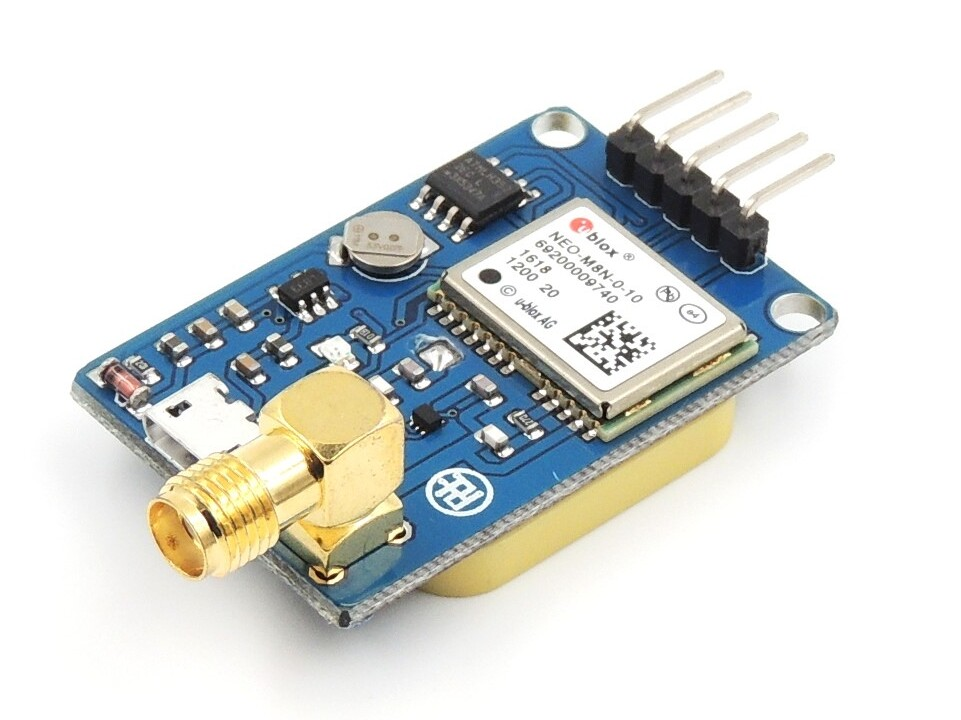
\includegraphics[scale=.4]{media/neo-m8.jpg}
    \caption{Development GNSS module u-blox NEO-M8}
    \textit{Source:} https://tutorials.probots.co.in/how-to-use-neo-m8n-0-01gps-module-using-u-center/
    \label{fig:neo-m8}
\end{figure}

Serial communication operates on the premise that both ends adhere to identical configuration settings. According to the official data sheet, the NEO-M8 module requires the following serial configuration:

\begin{itemize}
    \item Baud rate of \textbf{9600} bits/s
    \item \textbf{8} data bits
    \item No parity bits
    \item \textbf{1} stop bit
\end{itemize}

As per the datasheet specifications, upon powering the module, it commences transmitting data at a steady periodic rate of \textbf{1 second}, provided that the serial communication setup is configured correctly \cite{neo-m8-datasheet}. This data, adhering to the \textbf{NMEA} (National Marine Electronics Association) protocol, is transmitted as plain text NMEA messages. This format ensures compatibility and ease of integration with navigation and tracking systems, allowing for efficient communication and accurate retrieval of positioning information. There are numerous NMEA messages, each conveying a different kind of data in unique fields. NMEA messages have a fixed format; each starts with a dollar sign and a message identifier, followed by specific data fields. For example, in the \autoref{fig:gga-nmea-breakdown} below, an NMEA message of the GGA type (GPS Fix Data) is broken down into corresponding fields.

\begin{figure}[ht]
    \centering
    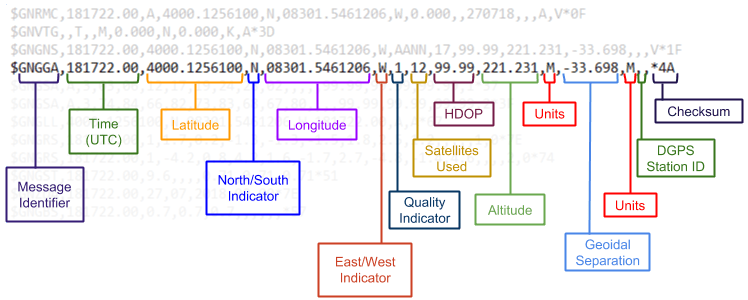
\includegraphics[scale=.6]{media/nmea-format.png}
    \caption{Breakdown of a GGA NMEA message}
    \textit{Source:} https://greenvillagedotblog.files.wordpress.com/2018/08/nmea-sentence2-e1533488080328.png
    \label{fig:gga-nmea-breakdown}
\end{figure}

The Message Identifier denotes the type of an NMEA message and the constellation used during the calculation process. The mapping of Talker ID codes (first two letters in the Message ID) to the different constellations is shown in \autoref{tab:nmea-talker-ids}. Note that this is not an exhaustive list of all the possible Talker IDs; included are only the main constellations that are mentioned in \autoref{subsec:constellations}.

\begin{table}[ht]
    \centering
    \begin{tabular}{|l|l|}
        \hline
        \multicolumn{1}{|c|}{Talker ID} & \multicolumn{1}{c|}{Constellation}     \\ \hline
        \textbf{GA}                              & Galileo                                \\ \hline
        \textbf{GB}                              & BeiDou                                 \\ \hline
        \textbf{GL}                              & GLONASS                                \\ \hline
        \textbf{GP}                              & GPS                                    \\ \hline
        \textbf{GN}                              & combination of multiple constellations \\ \hline
    \end{tabular}
    \caption{Mapping of Talker IDs and GNSS constellations}
    \label{tab:nmea-talker-ids}
\end{table}

As previously mentioned, a vast array of NMEA messages exists, making it impractical to describe each one in this document. Therefore, only the messages specifically sent by the NEO-M8 will be addressed herein, ensuring a focused discussion on relevant data formats and content. According to the datasheet, seven specific messages are enabled in this particular module by default. With the exception of the TXT message, their functions are described in \autoref{tab:nmea-neo-m8-default}.

\begin{table}[ht]
    \centering
    \begin{tabular}{|l|l|}
        \hline
        \multicolumn{1}{|c|}{Message ID} & \multicolumn{1}{c|}{Function}                                 \\ \hline
        \textbf{GGA}                     & Time, position, and fix related data                          \\ \hline
        \textbf{GLL}                     & Position data: position fix, time of position fix, and status \\ \hline
        \textbf{GSA}                     & GPS DOP and active satellites                                 \\ \hline
        \textbf{GSV}                     & Number of SVs in view, PRN, elevation, azimuth, and SNR       \\ \hline
        \textbf{RMC}                     & Position, Velocity, and Time                                  \\ \hline
        \textbf{VTG}                     & Actual track made good and speed over ground                  \\ \hline
    \end{tabular}
    \caption{NMEA messages sent by the NEO-M8 by default}
    \label{tab:nmea-neo-m8-default}
\end{table}

Each time the ESP receives an NMEA message, it must be parsed so the programmer can use the data. As parsing the messages manually would be quite cumbersome, a 3rd party library was brought in (more in \autoref{subsec:3rd-party-libs}).

\section{Firmware development}
Developing firmware for embedded systems like ESP32 differs from writing conventional code for desktop or web applications. The programmer has to be mindful of the resource intensity of their code. RAM and CPU usage play a big role, as does the size of the codebase itself; efficiency is key in embedded systems. Therefore, it is important that the programming language used is very low-level so as not to introduce much overhead. Languages like Java, Python, or JavaScript introduce a lot of overhead and increase the footprint of the software because they are more or less designed for good developer experience. On the other hand, C or Rust are very low-level counterparts that are great for writing embedded firmware. 

If the developer wanted to go even lower, they would arrive at ASM - the assembly language, where the individual instructions are the code. For larger applications using Assembly directly is very difficult and often impractical. The firmware for this project is written in \textbf{C++} as it offers enough low-level access to the hardware, introduces very little overhead, and has many QoL features over the basic C language.

\subsection{Development environment}
The IDE of choice during the development of this project was CLion from JetBrains in conjunction with the PlatformIO plugin. PlatformIO provides a convenient way to manage libraries in a project and greatly simplifies embedded development with its predefined project structure (as seen in \autoref{fig:firmware-project-structure}) and lifecycles. This project is considered a small one in the world of embedded development; thus, most of the directories generated by PlatformIO were unused. The directories used are the \verb|data| directory, where the front-end code is placed, so it can be uploaded to the flash memory using the command \verb|pio run --target uploadfs| and understandably, the \verb|src| directory containing the source code.

\begin{figure}[ht]
    \centering
    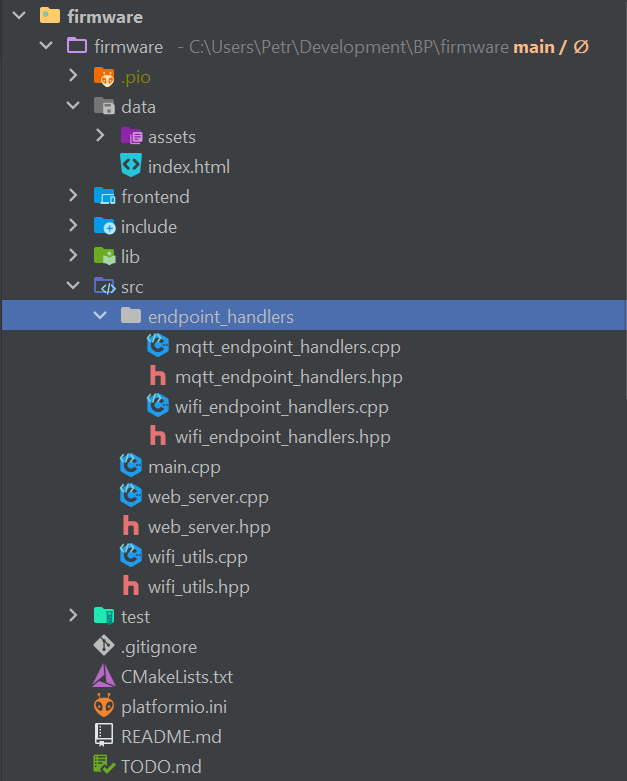
\includegraphics{media/firmware-project-structure.png}
    \caption{Project directory structure panel in CLion}
    \label{fig:firmware-project-structure}
\end{figure}

In embedded systems, particularly in real-time embedded systems, the main flow of the program often revolves around an infinite loop where the application's core logic resides. This loop typically iterates indefinitely, constantly checking and responding to various inputs, events, or conditions. Flags (or "status variables") are a crucial part of embedded programming. They serve as indicators or markers representing certain states or conditions within the system. These flags are frequently checked within the main loop to determine the course of action the program should take next. The programmer could create the whole base of an embedded system on their own, which is the usual route for bigger commercial code bases, but programmers frequently choose the Arduino framework. It abstracts away many of the low-level hardware details and exposes a convenient entry point for the programmer. The code listings below depict the difference between a standard C and an Arduino-style program. 

\begin{lstlisting}[language=C, caption=Ordinary C program, captionpos=b]
int main() {
    // code
}
\end{lstlisting}

\begin{lstlisting}[language=C, caption=Arduino style C program, captionpos=b]
void setup() {
    // setup, initialization, etc.
}

void loop() {
    // code to be executed continuously
}
\end{lstlisting}

The Arduino framework exposes two methods. The \verb|setup| method is where the program's initialization happens and usually includes setting up pins and communications. The other \verb|loop| method is where the code that runs continuously many times a second is placed.

\subsection{3rd party libraries}
\label{subsec:3rd-party-libs}
The base Arduino framework integrates many different libraries, most notably the \textbf{WiFi} library for interacting with WiFi networks and \textbf{LittleFS} to help traverse and interact with the file system. Configurations needed to survive restarts, so they had to be stored in flash storage. \textbf{Preferences} library provides ESP32-compatible Preferences API for various platforms. Numerous other 3rd party libraries were used throughout different parts of the firmware during development.

The microcontroller needed to run its own web server to expose a web application for configuration purposes. A library called \textbf{ESPAsyncWebServer} is a popular and reliable library that simplifies setting up an asynchronous HTTP and WebSocket server.

As the web server exposes an API, working with JSON would eventually become inevitable. Because using string concatenation as a poor man's JSON framework was out of the question and the C++ standard library doesn't natively support JSON, the \textbf{json} library by Niels Lohmann was leveraged.

For parsing NMEA messages received from the GNSS module, the \textbf{TinyGPSPlus} was used. Like its predecessor, TinyGPS, this library provides compact and easy-to-use methods for extracting position, date, time, altitude, speed, and course from consumer GPS devices \cite{tinygpsplus}.

Data is transmitted from the microcontroller using the MQTT protocol. The microcontroller needed to construct and publish an MQTT message to a specific topic (\verb|esgps/gnss|). Once more, a library designed for this purpose was utilized, specifically the \textbf{PubSubClient} library.

A few hardware-related libraries were also used. The solution contains a button for toggling the WiFi hotspot. Implementing a button is not terribly difficult, but it certainly has some caveats. One of the major problems was button bounce. A library called \textbf{ezButton} was able to abstract all issues away and expose a simple API for the developer to use.

The accelerometer and gyroscope module also required special handling, as it communicates over the I2C bus. The \textbf{MPU6050} library alongside \textbf{Wire} made integrating the module into the solution simpler by abstracting away handling the raw packets.

\subsection{Configuration web interface}
The configuration web interface will most likely be used once or twice throughout the device's lifetime, mainly for initial configuration. Therefore, the front end did not need to be extra sophisticated but purely functional, i.e., the reason for its simplistic design (as seen in \autoref{fig:config-interface-esp}). The application was once again built with the VueJS framework. In this case, though, the CSS library of choice was \textbf{Bootstrap}.

The application allows users to configure the device in different areas. The main configuration necessary is the details for the MQTT broker, specifically the address of the server and the port (1883 by default), along with the login credentials. Furthermore, the microcontroller must be connected to WiFi, so a WiFi manager was implemented. It lists all available networks in the near vicinity with their respective RSSI values. The user can connect to any one of the networks, assuming a correct password is entered.

A GNSS debug section is also implemented, where raw GNSS data can be inspected if something is out of the ordinary so a conclusion can be drawn.

\begin{figure}[ht]
    \centering
    \frame{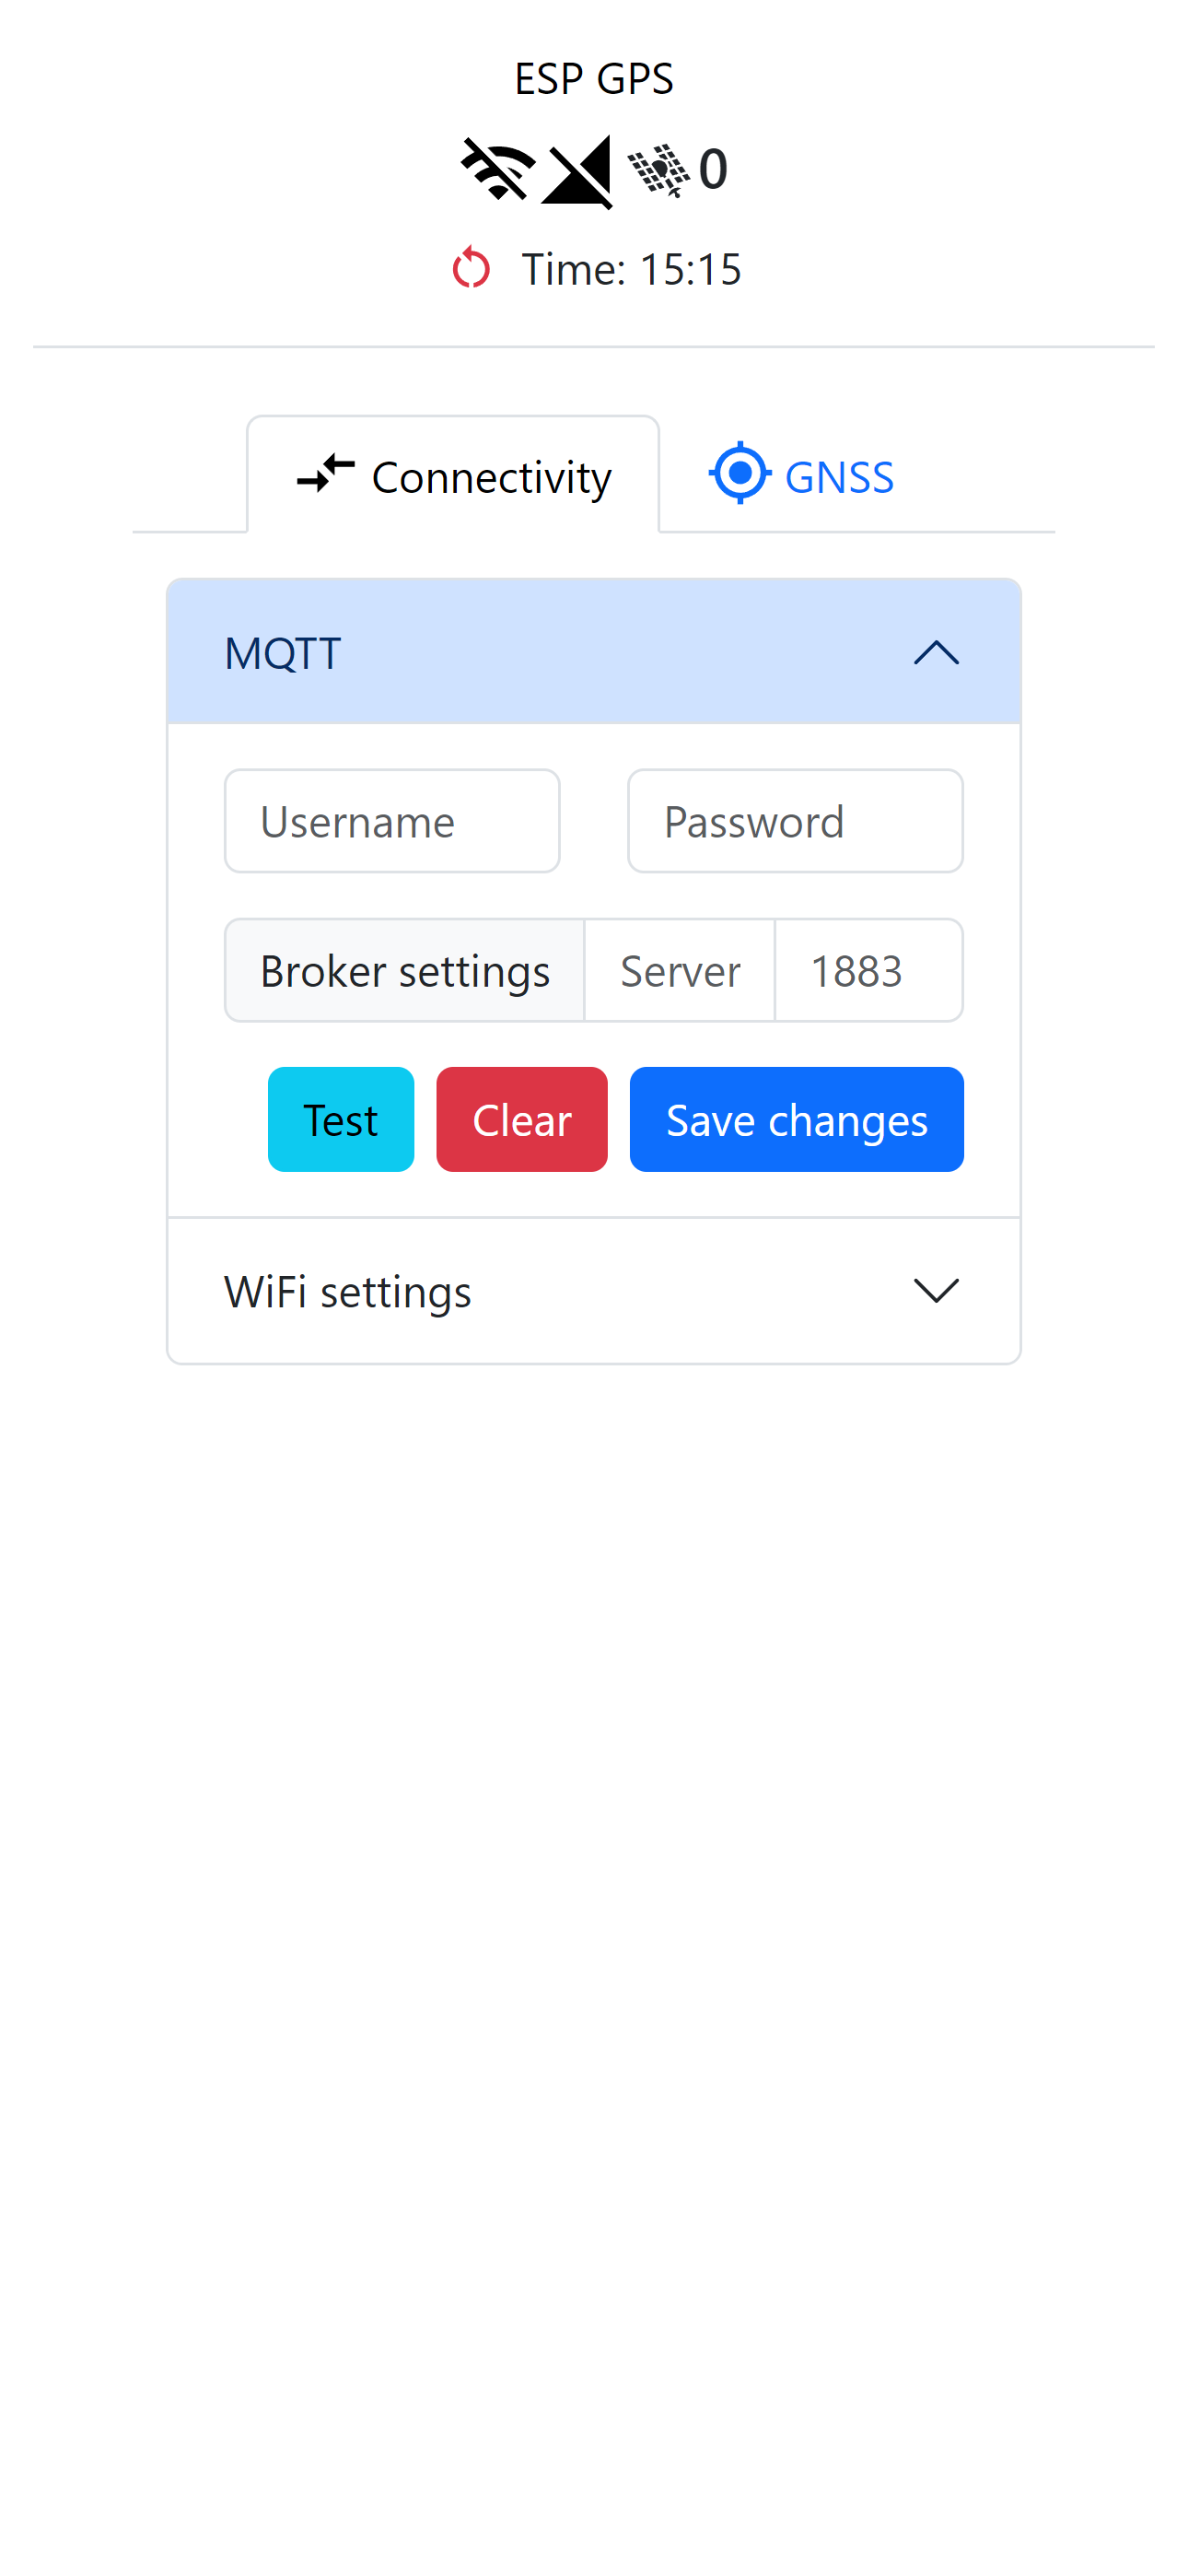
\includegraphics[scale=0.21]{media/esgps_esp32_config_gui.png}}
    \caption{Configuration web interface (iPhone 14 Pro Max)}
    \label{fig:config-interface-esp}
\end{figure}

After the front-end application reached its final state, the build process followed. Vite builds the Vue application into three files - \verb|index.html| and the CSS and JavaScript bundles.

\chapter{Web application}
\label{chap:application}
Now that the positional data has been gathered and sent, the next piece of the puzzle revolves around the web application. This application is constructed using a client-server architecture. 

This chapter is divided into two primary sections. The first, \autoref{sec:back-end}, delves into the application's back-end, exploring various technologies and problem-solving approaches. In the subsequent section, \autoref{sec:front-end}, we delve into the development intricacies of the user interface, along with considerations for enhancing user experience and ensuring seamless interaction with the system. 

From database management to user interface design, this chapter provides a comprehensive overview of the development process for both the back-end and front-end components of the web application.

\section{Back-end}
\label{sec:back-end}
The supporting back-end has multiple crucial responsibilities, the most significant of which are the following:

\begin{itemize}
    \item Processing subscribed GNSS data 
    \item Middleman between the presentation and the data layer
    \item Authentication and authorization
\end{itemize}

\subsection{The Spring framework}
As of April 2024, this project is using the Spring Framework 6. It provides a comprehensive programming and configuration model for modern Java-based enterprise applications - on any kind of deployment platform. At its core lies the Inversion of Control (IoC) container, which manages object instantiation and configuration, promoting loose coupling and facilitating easier testing. Dependency injection is also a key concept, enabling the injection of dependencies at runtime and enhancing modularity and maintainability. Aspect-oriented programming (AOP) aids in separating cross-cutting concerns from core business logic, leading to cleaner code. Spring offers a magnitude of different modules, which extend its capabilities.

\subsection{Data persistance}
When it comes to storing data, there are multiple paths the developer can take. Most notably, data is stored in files or a database. Storing data in files is a common practice for smaller applications where performance and scalability are not among the main concerns. Pretty much all desktop applications store their data in files. If each installed application ran its own database, the computer would quickly run out of resources because of the overhead databases introduce. In the case of web applications, the common practice shifts towards using databases for storing data. Unlike desktop applications, where each program may handle its own data in separate files, web applications often deal with larger volumes of data and require concurrent access by multiple users. Databases offer several advantages, including efficient data storage, scalability, concurrent access, and transaction support. Additionally, databases provide features like indexing, querying, and data integrity constraints, which are essential for managing complex data relationships and ensuring data consistency. Therefore, web developers typically opt for databases, such as MySQL, PostgreSQL, MongoDB, or others, to store and manage their application data effectively.

Choosing a database really depends on the specific needs of the application. This project relies on a document-based database. In this project, a decision had to be made between an SQL and a document-based database. Ultimately, it came down to the data structure and specific features required by the application. One of the benefits of document-based databases is that there isn't a need for a set data structure. Each record, a document, can have a different structure and contain a special data set. The most notable benefit that MongoDB brings to the table is the native support of time-series data. Time series data refers to a sequence of data points collected or recorded at successive and equally spaced intervals over time. For this project, numerous data points will accumulate throughout the application's lifespan, necessitating precautions to ensure the application's future resilience. MongoDB offers several handy features for managing time-series data, including data expiration. With this feature, each collection can define a specific duration after which data points expire. This capability is fundamental across most time-series databases, preventing storage overflow by automatically removing outdated data.

The Spring framework, particularly the Spring Data module, greatly facilitates data management and database interaction. An initial step involves defining models, each representing a distinct entity. For example, in this scenario, separate models are created for a data source and for individual data points. These models are typically expressed as Java classes or records, enhanced with annotations. These annotations assist the Spring Data module in interpreting the purpose of the defined fields; for instance, \verb|@ObjectId| signifies the ID field, aiding in contextual understanding and streamlined data handling. Instances of these model classes will later represent individual records in the database.

The concept of repositories is also quite important, as these repositories (in the code defined as interfaces that extend the parent \verb|Repository| interface from Spring Data, in this case, \verb|MongoRepository|).

\subsection{DTOs}
The concept of DTOs (Data Transfer Objects) is quite simple but proves powerful as applications grow. Put simply, the server should treat the model class as an internal tool that shouldn't be exposed to the users. For instance, the \verb|User| model class contains fields that are not desirable to be seen by users (mainly the password hash, as it serves no purpose to the user and, more importantly, poses a security risk).

The conversion from a model instance to a DTO usually happens at the controller layer. Services return the internal model instances, and the controllers are responsible for presenting the data to the user. This is the recommended flow by the Spring developers.

\subsection{Security}
Security is a big part of any modern web application. There are many aspects that go hand in hand to provide a secure user experience and prevent bad actors from getting ahold of sensitive user data. 

Something all web application developers have to deal with is \textbf{session management}. Once a user successfully authenticates, a session is established, and it falls upon the developer to handle it securely. In the old days, developers usually handled all the session logic themselves. Nowadays, though, with the plethora of frameworks to choose from, this task is usually already handled by the framework of choice. This is a good thing because it saves time, thus greatly increasing effectiveness and improving security, as the great minds behind these frameworks usually specialize in cybersecurity. Therefore, they can handle it much more securely than an average programmer. This is where Spring Boot comes in. Amongst its dependencies, Spring Session resides. Thanks to this dependency, Spring takes care of the whole process with the help of session cookies. A session cookie is a small piece of data stored by the user's browser during their session on a website. Unlike persistent cookies, which are stored on the user's device for a specified duration, session cookies are temporary and are typically deleted once the user closes their browser. This cookie is sent with every request to the server. During the authentication phase, Spring Security can detect the session cookie. If the session remains valid, it proceeds to authenticate the user (more about authentication in \autoref{subsec:auth}).

Another crucial aspect of overall security is \textbf{CORS} (Cross-Origin Resource Sharing), which pertains solely to the application's usage within a web browser. CORS imposes restrictions on which domains can send requests to the backend server. Consequently, the server must receive the domain information beforehand to shape responses accordingly (more on this in \autoref{sec:deployment}). This is accomplished through the use of headers, enabling the server to regulate access based on the specified domains.

\subsection{Authentication}
\label{subsec:auth}
This project required some integration headroom, which meant multiple ways to authenticate needed to be implemented. The usual flow of user authentication on the front end of the application is as follows:

\begin{enumerate}
    \item User opens up the applications and, depending on whether they already have a valid session established, are prompted with a sign-in form
    \item After the user fills in their credentials and submits the form. The credentials are packaged into a JSON payload that is sent to the server using an HTTP POST request to the authentication endpoint (in this case \verb|/auth/login|)
    \item The custom filter \verb|JsonUsernamePasswordAuthenticationFilter| will extract the credentials and use an \verb|AuthenticationManager| (more specifically the \verb|ProviderManager|)
    \item As \verb|ProviderManager| itself doesn't authenticate anything; it delegates it to the \verb|DaoAuthenticationProvider|, which will attempt to look up the user in the database and use the password to authenticate the request
    \item If the authentication was successful, the server returns status \verb|200| along with the session cookie. On the off-chance the server couldn't authenticate the request, it will return status \verb|4xx|, depending on what went wrong
\end{enumerate}

The general authentication flow is depicted on \autoref{fig:ss-auth}. 

\begin{figure}[ht]
    \centering
    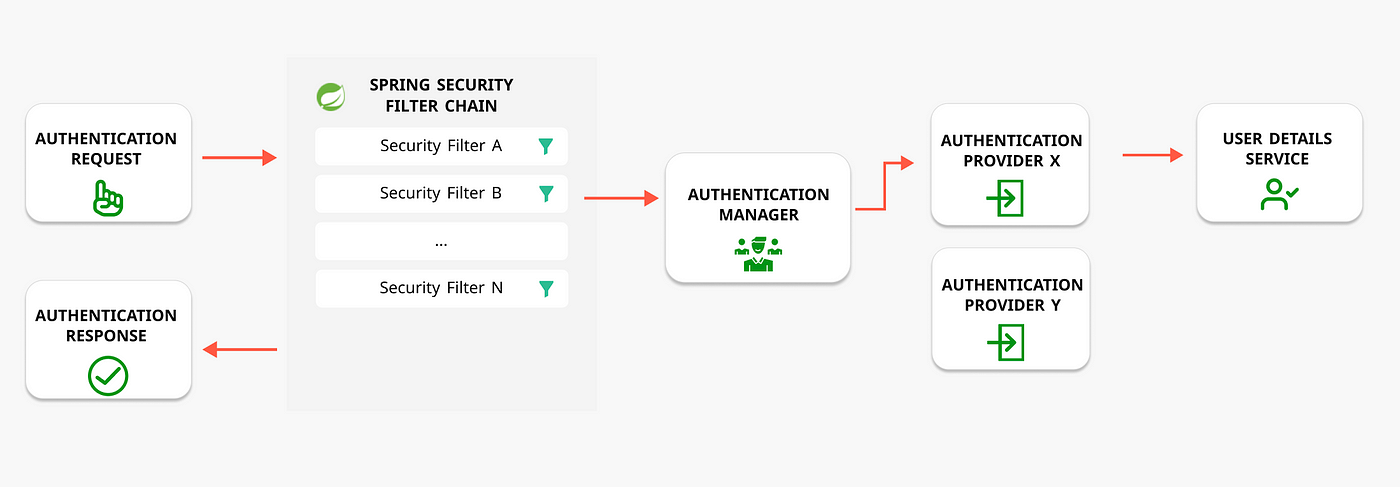
\includegraphics[scale=.33]{media/spring-security-auth.png}
    \caption{Authentication flow in Spring Security}
    \textit{Source:} https://kasunprageethdissanayake.medium.com/spring-security-the-security-filter-chain-2e399a1cb8e3
    \label{fig:ss-auth}
\end{figure}

As mentioned above, as this would be the sole authentication entry point, another option needed to be implemented. The \textbf{API key architecture} was selected as the other authentication method. Its simplicity of implementation, coupled with the powerful possibilities it brings to the table, made it the perfect candidate for the task at hand. Implementing API keys was relatively straightforward, thanks to Spring Security and its infinite extensibility. Still, it requires a brief description as there are many moving parts and Spring Security specific terminology. 

A custom authentication filter was plugged into the security filter chain. This filter is applied to every request, checking whether the \verb|Authorization| header is present and contains a value. It also requires the value to be a \textit{Bearer} type token (in simple terms, the value of the header has to have the word "Bearer" as a prefix with a space separating the two). Once such a request is found, the filter again hands the authentication responsibility to an \verb|AuthenticationManager|. The \verb|AccessTokenAuthenticationProvider| attempts to look up the given API key in the database. If the key is present in the database, it is considered valid and only needs to be checked for a few things before successfully authentication. More specifically, the provider needs to make sure that the token isn't disabled or expired.

\subsection{Authorization}
After authentication comes authorization. The server verifies the user's identity, and then comes the question, "Is this user allowed to perform a specific task?". Again, Spring Security was heavily leveraged to tackle this issue. Basically, two user groups were created (in Spring Security referred to as \textbf{Roles}) - \textbf{User} and \textbf{Administrator}. This provides a simple enough separation of concern but still allows for decent permission granularity.

In this application's security configuration, access to endpoints is restricted through a combination of URL and HTTP method-matching logic along with user role comparisons. This approach ensures that only authorized users with the appropriate roles can access specific endpoints.

\subsection{Real-time data communication}
In many modern web applications, there is often a need for real-time changes to the web interface. Most notably, these include notification pop-ups or loading mechanics (spinners, progress bars, etc.). This application, too, had to implement some of the mentioned elements in order to improve the UX (User Experience). In particular, a notification system had to be put in place to notify administrators when a new data source becomes available and is ready for adoption. Additionally, the dashboard's main function is to display live activity on a map. This location data must be transmitted to the front end in real-time. There are several different techniques to tackle the issue of data streaming, and all have their respective advantages and disadvantages.

The simplest way to emulate real-time functionality is to poll the server for information continuously. HTTP polling, more often than not referred to as \textbf{short polling}, is based on continuously sending HTTP requests to the back-end every so often. This technique is perfect when accuracy doesn't play a big role, as the speed at which new data can be presented to the user depends solely on the polling period, which, in this case, is the main parameter to be carefully chosen. Using a long polling period will result in the appearance of lag because new data might be waiting to be polled at any point. On the other hand, a really short period may be quite resource-taxing, as each request requires creating a new TCP connection. As the client base grows, so does this problem. With more users polling data simultaneously, the volume of requests escalates, inevitably pushing the server's bandwidth and hardware resources to their limits. In this instance, the notifications needed to be quite accurate, ideally to the second. All active sessions polling the server every second at the same time wasn't really a scalable solution.

\textbf{Long polling} presents a compelling alternative to short polling by addressing some of its key limitations. Unlike short polling, which relies on frequent requests to the server regardless of data availability, long polling adopts a more efficient approach. Long polling minimizes unnecessary requests by initiating a connection and waiting for a response only after a successful data exchange, thereby reducing server load. It facilitates real-time updates between the client and server, ensuring prompt new data delivery. Its simplicity and compatibility with standard HTTP protocols make it accessible and widely supported. However, long polling introduces latency as the client waits for responses, and it can consume server resources, particularly under heavy loads. Managing long-lived connections and handling browser limitations require careful consideration. 

Traditional methods of achieving real-time communication in web applications often involve makeshift solutions that can be considered somewhat hacky. However, purpose-built technologies tailored for this task offer more robust and efficient solutions. One such widely embraced technology is \textbf{WebSockets}. WebSockets is a communication protocol that provides full-duplex communication channels over a single, long-lived TCP connection. Unlike traditional HTTP connections, which are typically stateless and request-response based, WebSockets enable bidirectional, real-time communication between clients and servers. Once established, a WebSocket connection remains open, allowing the client and server to send messages asynchronously. 

WebSockets are frequently utilized in real-time chat applications. However, for straightforward unidirectional communication tasks, WebSockets can be overly complex and resource-heavy. This is where \textbf{Server-Sent Events} (SSE) step in, offering a simpler alternative. Unlike WebSockets, SSE is plain HTTP with a very specific \verb|Content-Type| header. For SSE to work, the header's value has to be set to \verb|text/event-stream|. After the request is sent, the connection stays open for as long as the client needs. This creates a one-way channel to which the server can push data. 

\begin{figure}[ht]
    \centering
    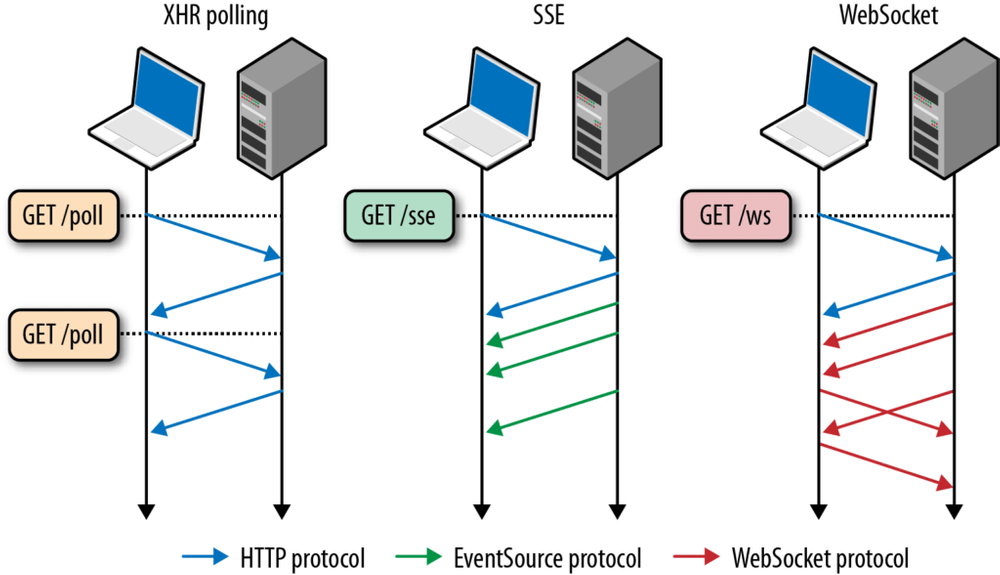
\includegraphics[scale=.4]{media/real-time-technologies.png}
    \caption{Different real-time communication technologies}
    \textit{Source:} https://tech.durgadas.in/real-time-events-websockets-vs-server-sent-events-8e92b94c6cc5
    \label{fig:real-time-technologies}
\end{figure}

In summary, there is a plethora of various options when it comes to real-time communication. Each one has advantages and disadvantages, and their use highly depends on the specific project (as seen in a brief pictographic illustration in \autoref{fig:real-time-technologies}). In this case, server-sent events perfectly fit the bill for this project and are thus employed repeatedly.

\subsection{Processing MQTT data}
After the application starts, it looks for the MQTT configuration in the database. More specifically, it looks for a document in the \verb|configurations| collection with the ID value of "mqtt" (such configuration document can be seen on \autoref{fig:mqtt-config}). After loading the configuration, the server connects to the MQTT broker using the configured parameters. A library had to be brought in to handle everything related to MQTT, specifically the Spring Integration MQTT module, which uses the Eclipse Paho MQTT implementation under the hood. The application keeps a connection to the MQTT broker alive so it can respond to any new messages immediately. In the event that the configuration isn't present in the database, which is also the initial state after the application is first deployed, the application logs it and continues to boot up as usual.

\begin{figure}[ht]
    \centering
    \frame{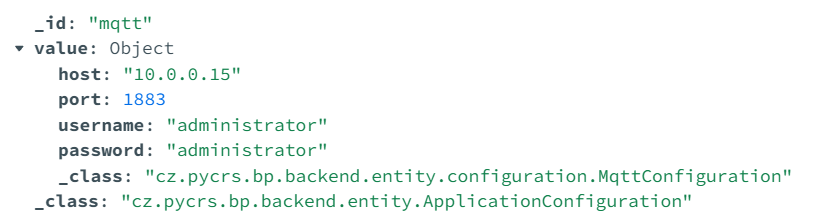
\includegraphics{media/mqtt-mongo-config.png}}
    \caption{MQTT configuration document}
    \label{fig:mqtt-config}
\end{figure}

The general algorithm (represented as a flowchart in \autoref{fig:mqtt-processing-algorithm}) is simple. When a new message is received, the application first extracts the source MAC address and attempts to look up the data source instance associated with it in the database. If unsuccessful, a new data source is created with that MAC address, inserted into the database, and returned for intermediate use. Conversely, if the MAC address is already associated with an existing data source, the respective instance is directly returned for further processing. 

Before proceeding with the algorithm, it is crucial to understand the concept of "adoption," which is a key aspect of data sources. Similar to the process observed in the Unify ecosystem, where all network devices undergo discovery by the central controller application upon network introduction, subsequent adoption by the administrator is necessary for their practical use. Data sources in this application follow the same principle. 

Once a data source instance is acquired, its adoption status is examined. If the data source is flagged as adopted, a new \verb|DataPoint| is generated with the values supplied in the original MQTT message. This data point is then linked to the relevant data source and inserted into the database. Furthermore, if any active sessions are subscribed to this specific data source, the newly created data points are dispatched to them using SSE to facilitate real-time map updates. If the data source has not yet been adopted, the processing stops at that point.

\begin{figure}[hp]
    \centering
    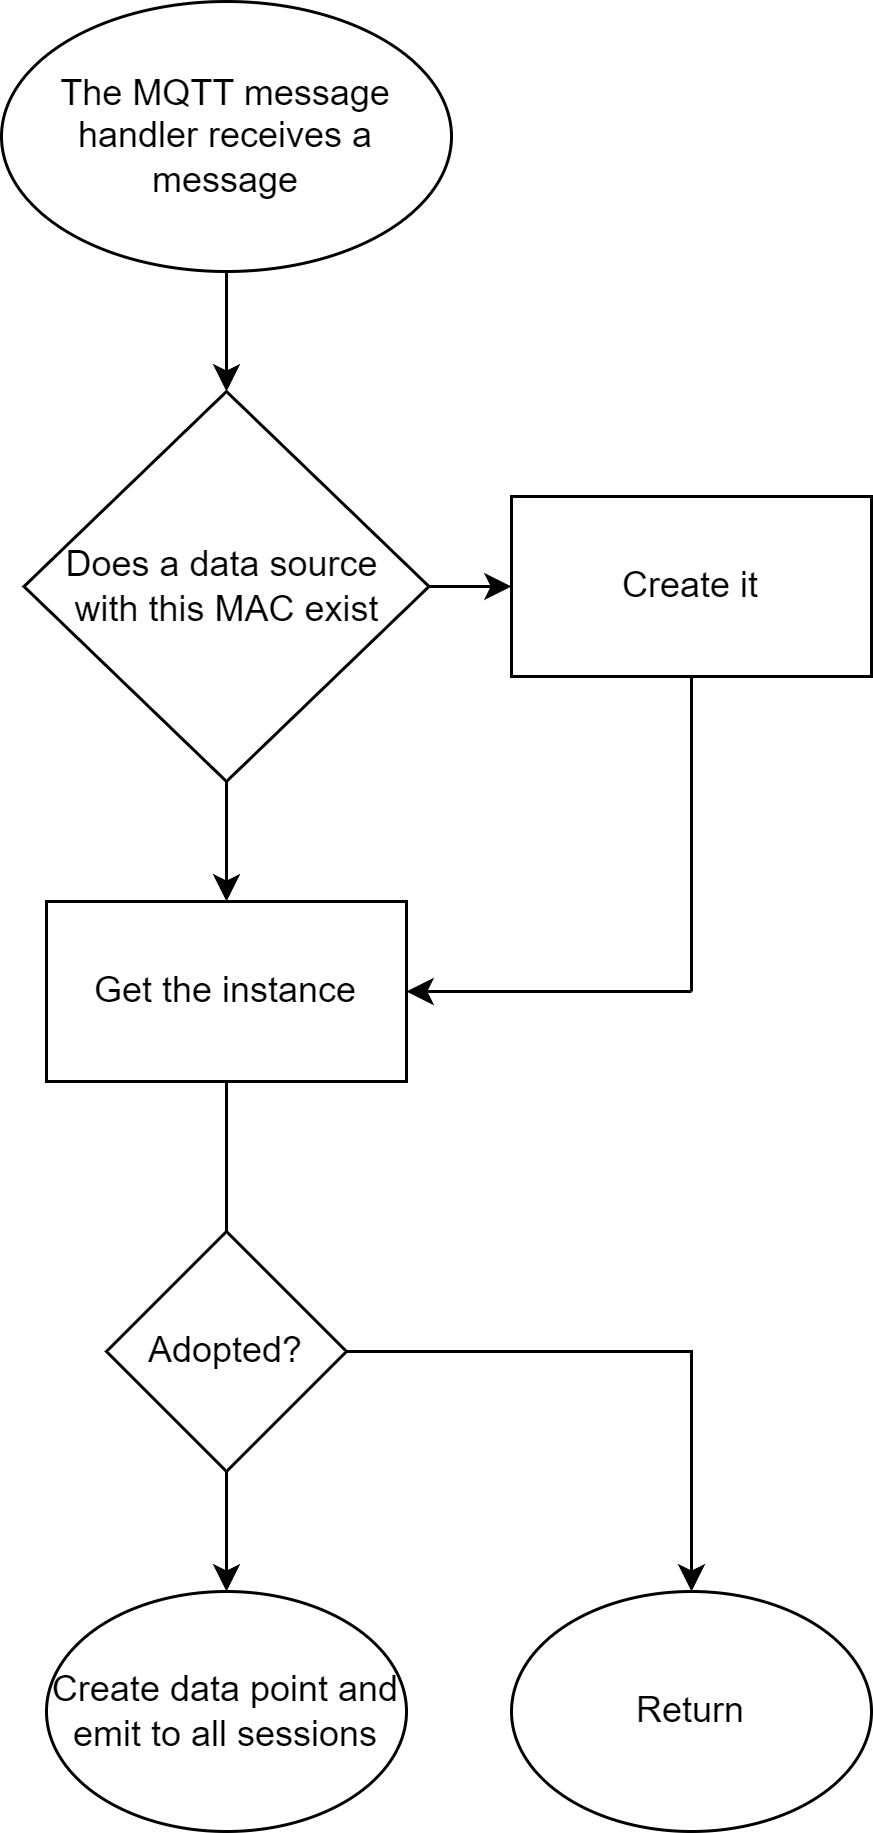
\includegraphics[scale=.32]{media/mqtt-processing-flowchart.png}
    \caption{MQTT message processing algorithm}
    \label{fig:mqtt-processing-algorithm}
\end{figure}

\newpage

\section{User interface}
\label{sec:front-end}
The application's front end, which users interact with, is written in JavaScript using the VueJS framework. In this section, all the important components and approaches will be outlined and described. 

During development, the \textbf{Vite} frontend tooling was used to serve the application. During deployment, Vite builds the application, and the files are then containerized. The front-end container also runs its own Nginx to serve the files, making the application available on port 80. More on this in \autoref{sec:deployment}.

\subsection{VueJS}
As mentioned, the front end is written in JavaScript using the VueJS framework. The framework's capabilities can be expanded with the help of plugins. This application uses several, the main ones being the \textbf{Vue Router} and a store library and state management framework \textbf{Pinia}.

Vue Router helps with managing multiple views in SPA (Single Page Application). The developer defines all the views as objects. These objects have certain required fields; more precisely, the \textbf{path} and \textbf{component} fields. These define what component is rendered at which URL. Each object can also have metadata. In this application's case, these are used for multiple reasons. Some views are only meant for anonymous users (i.e., users not yet signed in), which is what the \textbf{unauthenticatedOnly} metadata field is used for. The navigation is generated from the router view list, but some views need to be excluded from the navigation. The \textbf{nav} field is used precisely for this reason. UI-specific metadata like the icon and user role are also required for each navigation link.

Pinia takes care of storing data sent by the server. It also defines functions related to querying the data. Individual services call these functions throughout the application's lifecycle.

\subsection{The map}
A big part of the application is the map displaying the location data. There are multiple options, including Google Maps, OpenStreetMap, or \textbf{Leaflet}, which was ultimately chosen as the technology of choice. 

Leaflet is the leading open-source JavaScript library for mobile-friendly interactive maps. It has an intuitive API that greatly improves the overall developer experience on this front. When the application loads, the map view is set to cover the entire world. The browser prompts the user for location permission. If permission is granted, the map view adjusts based on the location returned by the Navigator API.


\subsection{Communication with the server}
An important aspect of any front-end application is reliable communication with the server. The simplest way to communicate over TCP or a Unix socket is the \verb|fetch()| function. It is ideal for very simple proof-of-concept projects. As the project grows, developers often opt for 3rd party libraries. The most popular tool for the job is the \textbf{Axios} library. 

Axios makes it simple to make many requests throughout the application. Firstly, an instance of Axios is created and configured with the necessary defaults (e.g., the API URL, credentials policy, etc.). The instance is then imported anywhere where requests need to be made. The appropriate functions (named according to their respective HTTP methods) are then used to execute the request. It is also built with JSON in mind, so executing requests where data needs to be transferred is straightforward.


\subsection{The design}
The application is laid out in a three-component manner (as depicted by a wire frame in \autoref{fig:app-wireframe}). At the top rests the \textbf{header bar} (often referred to as a navigation bar, but in this case, it doesn't really contain anything related to navigation) containing the logo on the left and the notification drop-down alongside the sign-out button on the opposing side.  Finally, the \textbf{main content} is placed in the remaining area.

\begin{figure}[h]
    \centering
    \frame{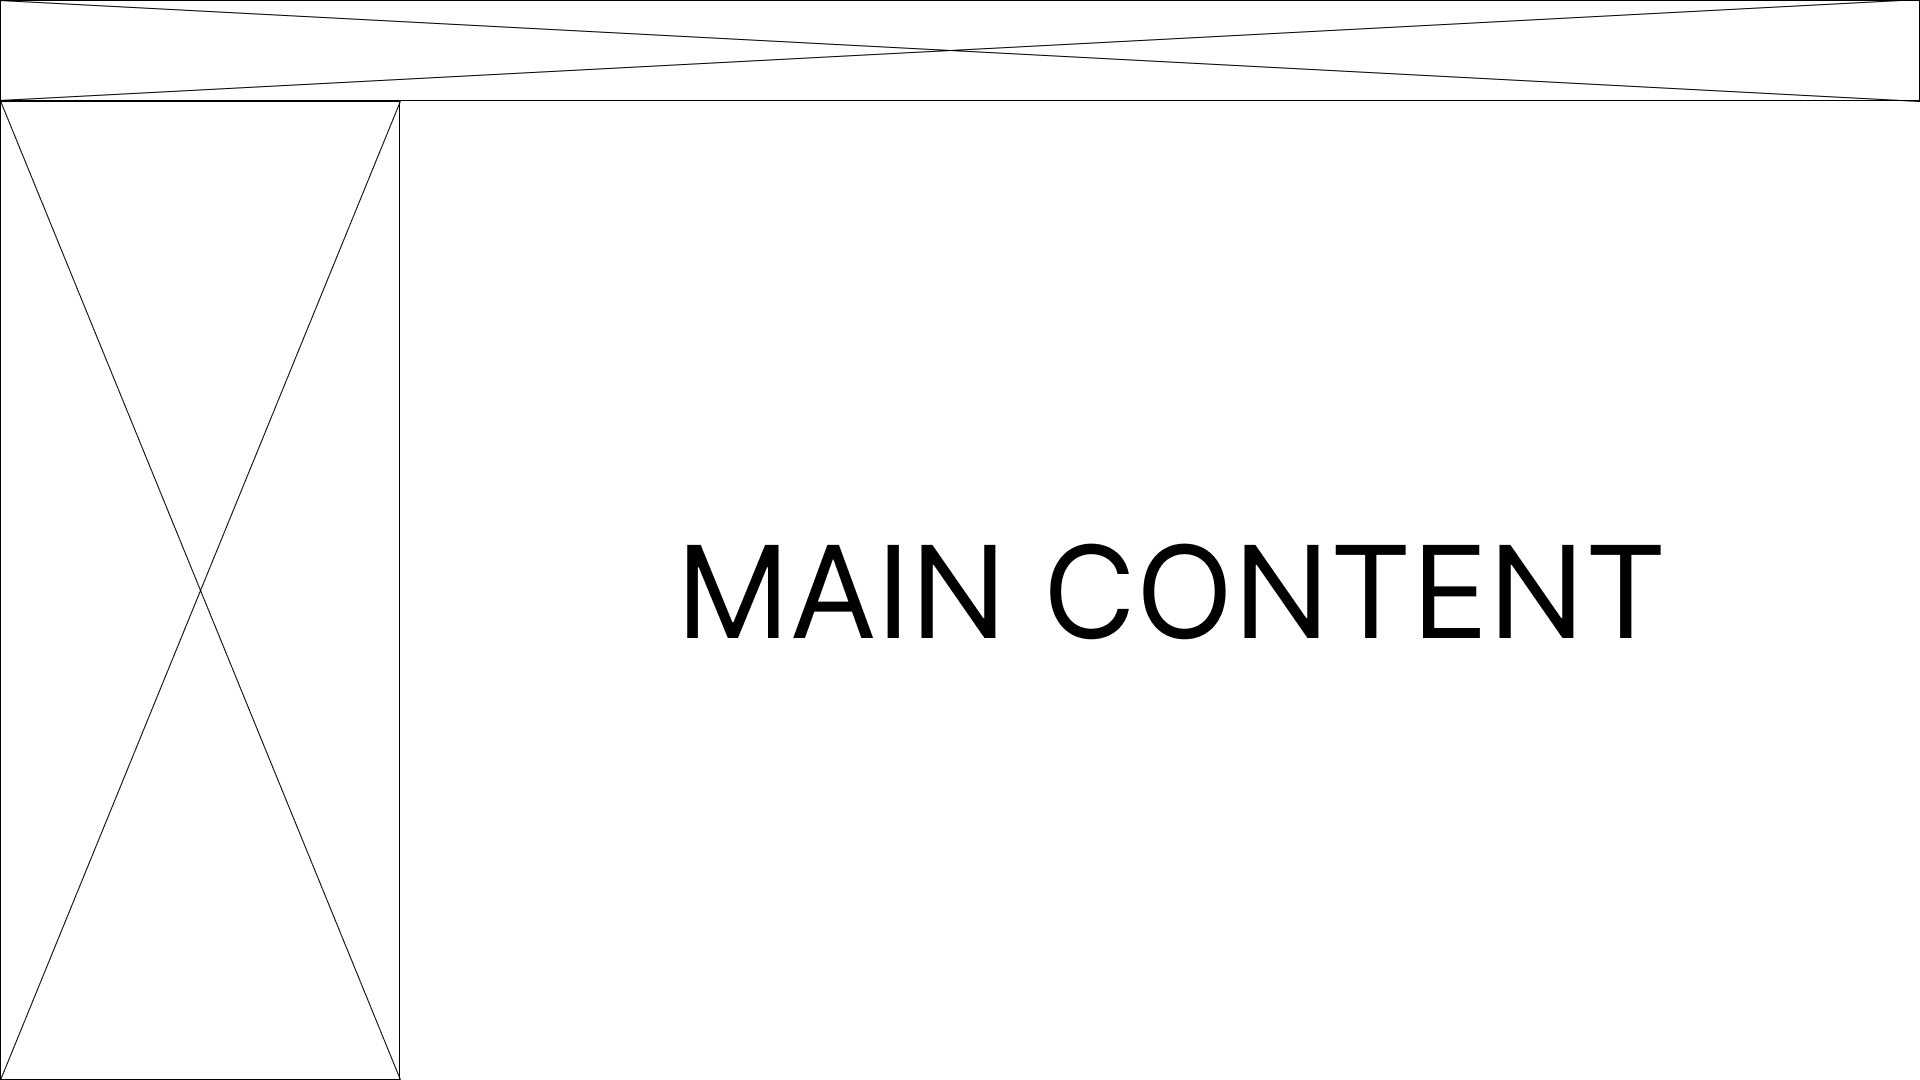
\includegraphics[scale=.22]{media/wireframe.png}}
    \caption{The application layout wire frame}
    \label{fig:app-wireframe}
\end{figure}

The main navigation part of this application is placed in the \textbf{left sidebar} (see \autoref{fig:sidebar}). It contains links that users can use to navigate throughout the application. The content of the navigation itself is dictated by the role of the currently logged-in user. Administrators have access to the application's full potential, whereas regular users are only permitted to a small set of features.

\begin{figure}[H]
    \centering
    \frame{
\includegraphics[scale=.5]{media/nav-sidebar.png}}
    \caption{The navigation sidebar}
    \label{fig:sidebar}
\end{figure}

From the perspective of UI, visual appeal plays a significant role in the attractiveness of any application. A visually appealing interface is pivotal for a successful product. Therefore, selecting an appropriate CSS library is essential. There are many excellent options available, such as Bootstrap, Tailwind, Materialize, Foundation, and others. In the case of this application, the \textbf{Bulma} library was chosen for several reasons, including the developers' familiarity with it.

Letting the users know the result of an action is really important for the overall UX. This is usually accomplished with some sort of pop-up notification. This application utilizes toast messages to solve this. According to \textit{uxpickle}, a toast notification is a non-modal, unobtrusive element to display a short message, and it appears on the screen when an event occurs \cite{toast-msg}. The \textbf{vue-toast-notification} library was used to simplify the implementation. A screenshot of such a notification can be seen on \autoref{fig:toast}.

\begin{figure}[H]
    \centering
    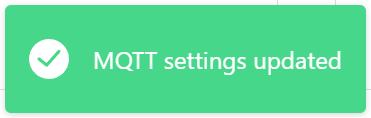
\includegraphics[scale=.75]{media/toast.png}
    \caption{Success toast notification}
    \label{fig:toast}
\end{figure}

The thesis appendix also dedicates \autoref{sec:app-screenshots} to showing off a handful of application screenshots.

\section{Deployment}
\label{sec:deployment}
The deployment strategy for this project is very common. All the components are containerized and orchestrated together. There are many options for containerization, like LXC, OpenVZ, and, most notably, \textbf{Docker}. Docker simplifies application deployment by separating its parts into standalone containers that run practically everywhere, no matter the hardware or operating system\footnote{Containerization using Docker is possible as long as the \textbf{docker engine} can be installed and run on that particular machine. Also, containers are usually tailored to a platform, i.e., x86, arm, etc.}. Thanks to Dockers' popularity and wide support, it, alongside \textbf{Docker Compose}, was selected as the deployment strategy of choice.

The final deployment was placed inside a preexisting infrastructure behind an additional reverse proxy (\textbf{Traefik}); the router definition can be seen on \autoref{fig:traefik-router}. It terminates the SSL/TLS connection and manages the Let's Encrypt certificates and their automatic renewals with ACME. 

\begin{figure}[ht]
    \centering
    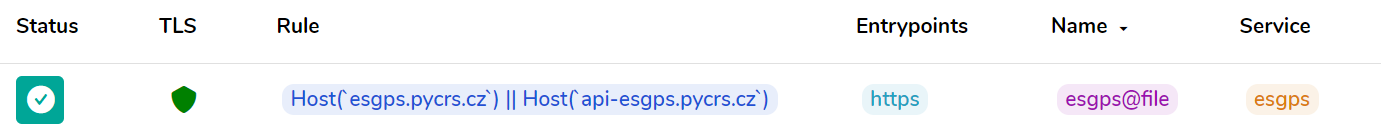
\includegraphics[scale=.65]{media/traefik-detail.png}
    \caption{Traefik router definition}
    \label{fig:traefik-router}
\end{figure}

The Docker Compose stack was deployed with the help of Portainer (\autoref{fig:portainer-stack-detail} shows the stack detail).

\begin{figure}[ht]
    \centering
    \frame{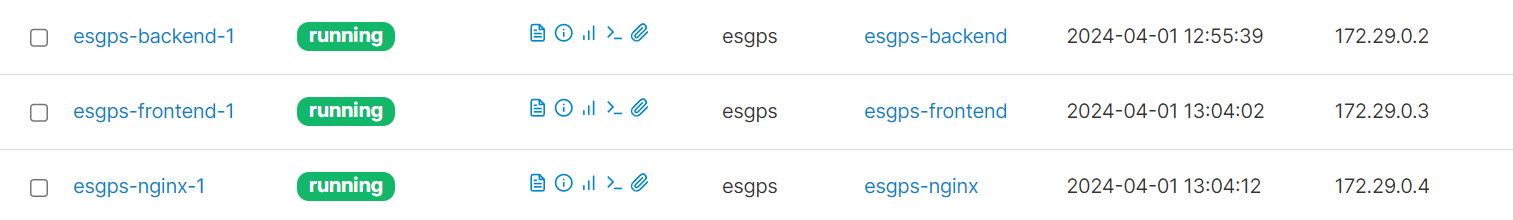
\includegraphics[scale=.6]{media/portainer-detail.png}}
    \caption{Stack detail in Portainer}
    \label{fig:portainer-stack-detail}
\end{figure}


\subsection{Walkthrough}
The deployment consists of \textbf{three} separate containers orchestrated together with Docker Compose (following the diagram in \autoref{fig:compose-structure}). The two main parts of the application (front-end and back-end) are separated into their own containerized environments as they each have different environmental requirements. The third piece of the deployment puzzle is a proxy handling user requests to the application. In this instance, a reverse proxy called \textbf{Nginx} was utilized. Based on domain matching, it is configured to serve the front-end application and route any API requests to the back-end container.

\begin{figure}[H]
    \centering
    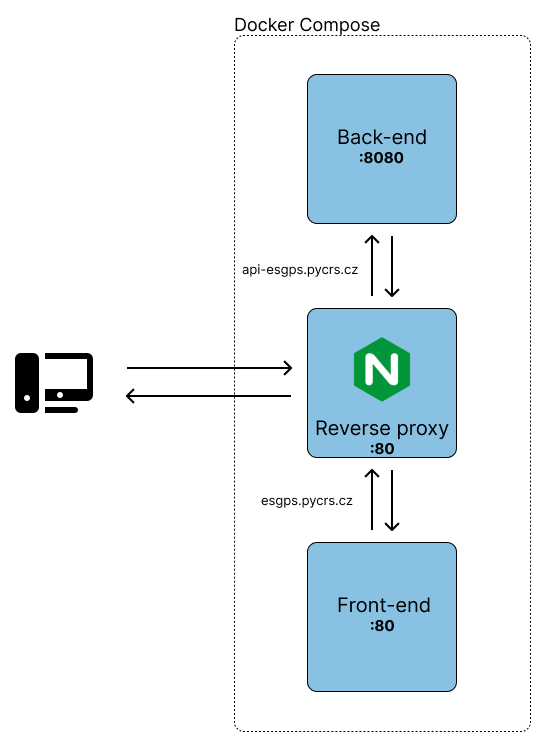
\includegraphics[scale=.6]{media/orchestration.png}
    \caption{The containerized infrastructure}
    \label{fig:compose-structure}
\end{figure}

The general process of deploying the application is as follows:

\begin{enumerate}
    \item Clone the repository
    \item Build the Docker images
    \item Create and run the container from the mentioned images
\end{enumerate}

Starting with getting the entire codebase, the administrator must clone the repository on their local computer or the deployment machine. As the \verb|git| version control system keeps track of changes, the \verb|git clone| command can be utilized to clone the repository. The following command will clone the repository over SSH into a directory called \verb|BP-app|.

\begin{verbatim}
    git clone git@github.com:Pzdrs/BP-app.git
\end{verbatim}

The repository contains a convenient \verb|docker-compose.yaml| file, which has the build contexts predefined to the repository structure; running this configuration with \verb|docker compose up| will bring up the whole application. Docker Compose will automatically build the images for all the containers with the help of Dockerfiles in each top-level directory. The domain and Mongo-related environment variables must also be changed to the specific deployment accordingly.

Another approach is to deploy without relying on containerization, opting instead to build from the source and run directly in the OS. This method entails a more intricate process involving setting up the environment and, ideally, running applications as Unix daemons. However, due to its complexity and the numerous possibilities for misconfiguration leading to issues, this process will not be covered.
\chapter{Results and testing}
\label{chap:results}
This final chapter preceding the thesis conclusion is dedicated to presenting the results. It summarizes the outcomes obtained from testing specific areas, providing ample space for their clarification.

\section{Storage implications}
\label{sec:storage-implications}
In a project of this nature, continuously collecting data and not deleting them, the logical thinking is that storage might become a problem in the future.

In the grand scheme, the only collection that will get considerably bigger is the \verb|datapoints| collection. Other collections, of course, take up space, but in order of kilobytes, which is negligible.

Each data point document is \textbf{119 bytes}. For 100,000 documents, the collection takes up \textbf{11.9MB} on disk (2.61MB compressed), which in today's world is not much. It is important to acknowledge that indexes also take up space. In this instance, the only indexed field is the \verb|_id| field. The index takes up 1.52MB on disk for the previously mentioned collection size. If multiple fields were to be indexed, the size would obviously grow.

It's also noteworthy that the collection can be configured as a time series, allowing for the setup of data expiry. This feature ensures the automatic deletion of old entries, thereby maintaining only a certain amount of historical information.

In conclusion, as the collected data points are not likely to reach 7-figure numbers or more, the storage likely does not need special attention.

\section{The impact of large time frames on performance}
Depending on the data distribution throughout time, larger time windows may require querying significantly more data points. 

Initially, the back-end server retrieves the desired data from the database. Subsequently, the data traverses through multiple layers before finally reaching the controller. Following this, it must be prepared into an HTTP response and dispatched to the client. While these steps may not consume significant time individually, their cumulative effect can be notable. This becomes more noticeable as the amount of data increases. 

The impact of increasing data points being queried is illustrated by \autoref{tab:time-impact-of-large-time-frames}. An exponential growth rate of base 10 capped at \textbf{10,000} data points was selected for testing, as this covered the usual workload the application may be subjected to.

In total, three distinct metrics were measured for every sample size\footnote{Tests were carried out exactly five times, and the results were averaged for the sake of consistency.}: the duration of the database lookup, the subsequent time required to transmit the HTTP response to the client over the network, and finally, the time to render the data on the map.

\begin{table}[ht]
\centering
\begin{tabular}{|l|l|l|l|l|}
\hline
                  & \textbf{10}  & \textbf{100} & \textbf{1000} & \textbf{10 000} \\ \hline
Database lookup   & \~{}0ms          & \~{}0ms          & \~{}0ms           & 2ms             \\ \hline
Network transport & 40.95ms          & 149.93ms          & 1352ms           & 13,6s             \\ \hline
Rendering         & 2ms          & 12.6ms          & 110.8ms           & 1090.6ms             \\ \hline
\textbf{Total (user perspective)}    & \textbf{35.4ms} & \textbf{171.4ms} & \textbf{1496.4ms}  & \textbf{15.1s}    \\ \hline
\end{tabular}
\caption{The impact of an increasing amount of queried data on different tasks}
    \label{tab:time-impact-of-large-time-frames}
\end{table}

From the table, it is apparent that the database does not contribute much to the overall time. MongoDB is an extremely well-optimized and performant piece of software, and considering the sample sizes, it is no surprise the time contributed is pretty negligible. At the 10,000 sample size mark, MongoDB's \verb|explain| tool returns non-zero \verb|executionTimeMillis| values. The execution time starts to matter when working with six-figure sample sizes. Querying 100,000 data points takes 23 milliseconds, a big jump from the previous.

\section{Economy analysis and cost breakdown}
As mentioned, this project is not backed by an organization or a funding entity. This means that during the hardware solution's design phase, each component's price had to be considered carefully. This, along with other less significant aspects, is the main reason for the proof-of-concept look of the construction. 

Designing and manufacturing a custom PCB is relatively affordable nowadays, but it still would be a significant added expense. The same applies to designing and 3D printing of an enclosure.

In the end, the solution's total cost came to roughly \textbf{735 Kč}. A detailed cost breakdown is provided in \autoref{tab:cost-breakdown}. The table shows that the most expensive part of the construction is the GNSS receiver. This is because a higher-end model (u-blox NEO-M8N) was chosen, offering features like multi-constellation support, ROM, and many more. Trailing behind, the ESP32 was the second most significant expense.

\begin{table}[ht]
    \centering
    \begin{tabular}{|l|l|}
        \hline
        \multicolumn{1}{|c|}{\textbf{Product name}} & \multicolumn{1}{c|}{\textbf{Price}}   \\ \hline
        GNSS module u-blox NEO-M8                             & 372 Kč          \\ \hline
        ESP32 development board                               & 207 Кč     \\ \hline
        I2C Gyroscope + Accelerometer module MPU-6050     & 77 Kč      \\ \hline
        No solder breadboard (830pin)                         & 57 Kč          \\ \hline
        Jumper wires                                          & \~{}20 Kč          \\ \hline
        LEDs  (red, green, blue)                              & \~{}2 Kč          \\ \hline
        Resistors (220Ω)                                      & \~{}1 Kč          \\ \hline
        Button                                                & \~{}1 Kč          \\ \hline
        \textbf{Total}                                        & \textbf{\~{}735Kč} \\ \hline
    \end{tabular}
    \caption{Products used in the construction of the hardware package}
    \label{tab:cost-breakdown}
\end{table}

\section{Data collection}
Typically, the RF power level received by an antenna on the ground will be between -125 dBm and -150 dBm \cite{receiver-sensitivity-testing}. When placing the hardware solution in the cabin of a car, due to the chassis being made out of metal, some signal issues were anticipated. An active antenna with a long enough cable was even purchased to be put on top of the car should there be any signal issues. 

After deploying the hardware solution in the top compartment of the dashboard so as not to obstruct the driver's view in any way (see \aref{fig:physical-incar-deployment}), it turned out that the receiver could pick up the signal without any significant problems; thus the antenna went unused.

\subsection{Sampling frequency}
Choosing an appropriate sampling rate affects multiple different areas of a given deployment. There are multiple implications that come with using a very high frequency:

\begin{itemize}
    \item Transmitting data very often might quickly eat through a data plan
    \item Even though it was concluded that the collected data does not take up very much space, writing to the database all day every day could be eventually harmful to the disk
    \item Displaying many more data points than necessary can cause significant lag to the web interface
\end{itemize}

During testing, all the collected data was sampled with the frequency of \textbf{1s} - the fastest sampling possible, as the GNSS module can't go any faster. This ensured the greatest detail and allowed for subsequent processing. The main testing lap had a standardized route (see \aref{fig:test-lap}) so that clear, unbiased conclusions could be drawn.

The effect of varying sampling frequencies is best demonstrated visually. \aref{fig:1s-samplerate} and \aref{fig:5s-samplerate} show the difference in detail captured with sampling frequencies of \textbf{1} and \textbf{5 seconds}, respectively. 

It is apparent that the slower frequency captures less detail, mainly the curvature. It could be argued that considering the not-so-perfect precision of the data coming from the GNSS module, this isn't really an issue. Due to the car's velocity at moderate speeds, the distance covered in between samples is quite small, minimizing the likelihood of missing significant detail. However, if we were to monitor an aircraft moving roughly 900 km/h, the scenario would necessitate a different narrative.

\section{Final thoughts}
It is always good to compare real-world results with the theoretical ideal outcomes. For this purpose, multiple routes were exported from Google Maps and imported into the application for comparison purposes. 

A portion of a route in Prague can be seen in \aref{fig:google-maps-export}. It is apparent that the data points are perfectly overlayed with the road and only in places where necessary (physical features of the rodes changing the curvature; a roundabout would be a perfect example).


\chapter{Possibilities of integration}
\label{chap:integration}
In the past, the general public desired so-called "plug-n-play" products more. People were not interested in tinkering or expanding the functionality of products they purchased. Fast forward to the year 2024 - the data age, open-source, versatility, and having options are things people value more and more. A fundamental principle of this project lies in its emphasis on expandability and future-proofing. Its open-source nature empowers developers to delve into its inner workings, identifying and rectifying bugs and even contributing new features. This collaborative approach invariably results in enhanced products that benefit all users.

One distinguishing characteristic of this project, setting it apart from the vast majority of similar solutions, is its approach to retrieving data from physical data sources. In accordance with the findings outlined in \autoref{sec:data-delivery}, a distributed messaging system served as the primary medium for data exchange, specifically employing the \textbf{MQTT protocol}. This distributed approach, which utilizes open-source, well-documented technologies, allows for simple troubleshooting and scaling down the line should the deployment grow in complexity; there is no proprietary technology that could render the deployment unusable in case of exponential growth. Expansion is feasible as long as devices gathering positional data can access the Internet and an MQTT server is accessible online. However, various other challenges may likely emerge before encountering potential bottlenecks with the broker. These could include issues such as network latency, device connectivity problems, or data processing bottlenecks.

Enabling access to the API for other systems is a feature that can significantly enhance the flexibility and expandability of a project. However, implementing this functionality may present a few challenges, particularly concerning authentication and authorization. Addressing such challenges offers a variety of approaches, spanning from straightforward methods like basic/digest authentication or API keys to more intricate yet versatile solutions such as OAuth, JWT, LDAP, and others. As previously established, \textbf{API keys} were used as the main authentication and authorization method for other systems interacting with the API. This choice was made due to its balanced combination of ease of implementation and sufficient security and flexibility. These keys are opaque tokens. Therefore, they do not require any special handling from the opposing system. A basic HTTP call with the key embedded in the Authorization header suffices for the API to provide data. This capability enables other systems to execute the same actions as the developed front-end solution. For instance, creating a platform for aggregating and analyzing collected data could be immensely beneficial for specific users. Additionally, developing a Home Assistant integration could seamlessly incorporate this project into an existing smart home system.

\chapter*{Conclusion}
\addcontentsline{toc}{chapter}{Conclusion}
A thorough problem analysis alongside detailed market research in both the software and hardware sphere was first carried out as a part of the thesis. A custom solution was designed and constructed based on the knowledge acquired in the analysis and research. The hardware portion of the solution was built on top of the ESP32 microcontroller and equipped with the u-blox NEO-M8 GNSS module. Furthermore, a gyroscope with an accelerometer module was used for optimization purposes. Lastly, several additional elements were integrated, specifically a WiFi hotspot control button and various indication LEDs.

A supporting web application was developed to view and manage collected data. The use of SSE (Server-Sent Events) allows users to view the live location of all data sources. Thanks to a MongoDB database, users also have access to historical data. The main entry point to the application is through the front-end dashboard, but thanks to the API token system, the REST API can also be leveraged for data access or integration into other systems.

The whole application was secured against the most common threats occurring on the web. The application was also packaged, containerized, and deployed using Docker. Thus, the application is fully functional and currently available at \href{https://esgps.pycrs.cz}{https://esgps.pycrs.cz}.

Regarding possible future improvements, developing and manufacturing a custom PCB may prove practical if the solution goes to market, which would decrease the price and simplify the deployment process for customers. Designing and 3D printing an enclosure would also be a logical next step.

\nocite{*}
\printbibliography[title={References}] % sazba seznamu citací 
\addcontentsline{toc}{chapter}{References} % vložení nadpisu do obsahu

\appendix
\chapter{Attachments}
\section{Source code}
The whole project is split into two GitHub repositories based on their scope. All source code related to the main web application is placed in a dedicated repository (back-end, front-end, deployment, utility Python scripts, etc.) available at \href{https://github.com/Pzdrs/BP-app}{https://github.com/Pzdrs/BP-app}. 

Consequently, the ESP32 firmware and the front-end code for the configuration interface is available at \href{https://github.com/Pzdrs/BP-firmware}{https://github.com/Pzdrs/BP-firmware}.

\section{Application screenshots}
\label{sec:app-screenshots}
\begin{figure}[htbp]
    \centering
	\makebox[\textwidth][c]{\frame{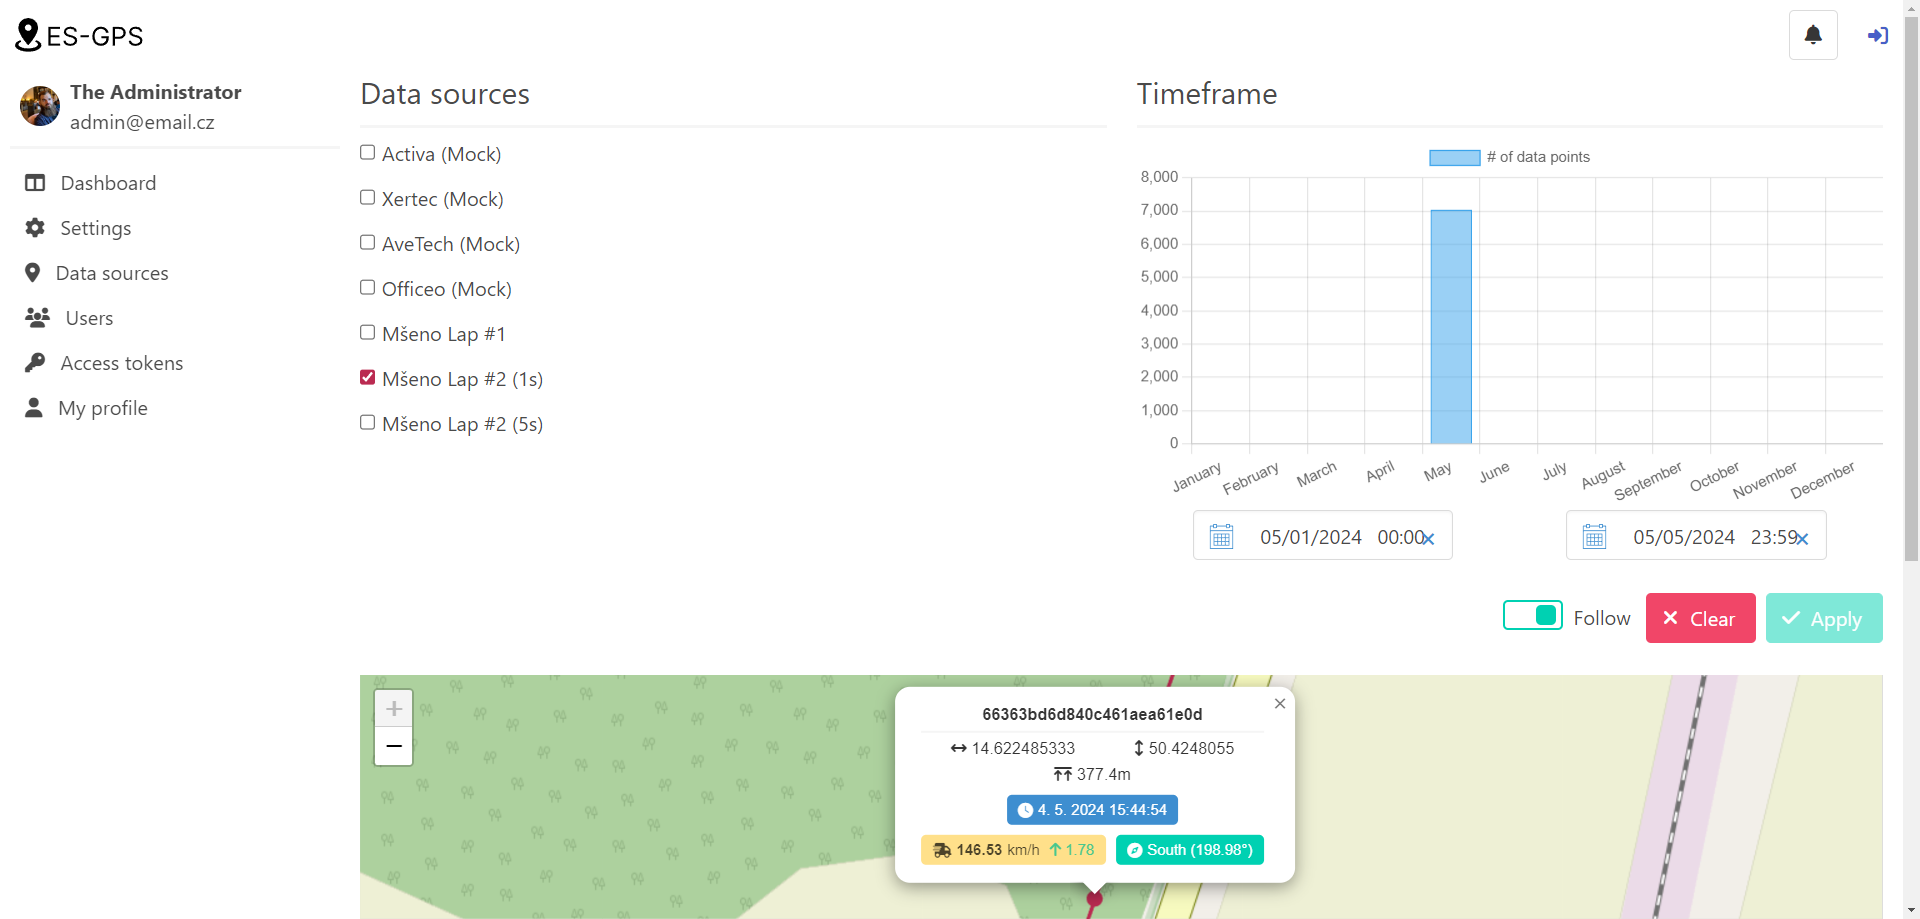
\includegraphics[width=1.2\textwidth]{appendix/preview.png}}}
    \caption{The main map view of the application}
\end{figure}

\begin{figure}[htbp]
    \centering
	\makebox[\textwidth][c]{\frame{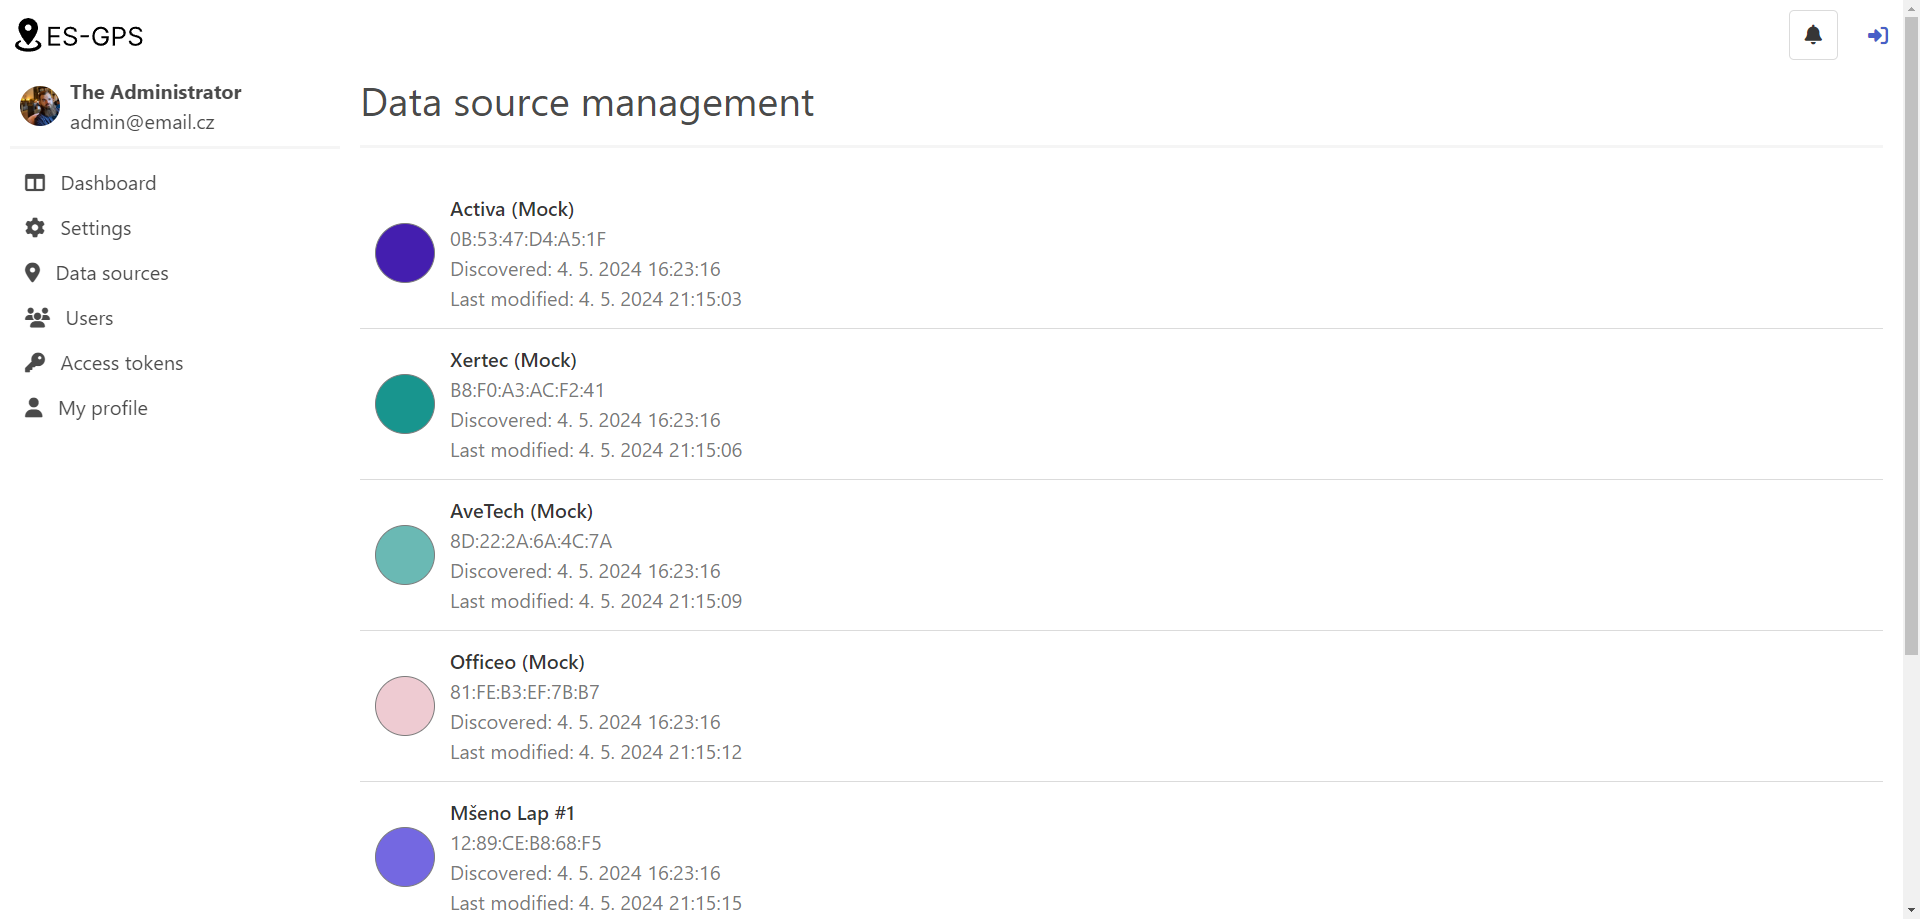
\includegraphics[width=1.2\textwidth]{appendix/data-sources.png}}}
    \caption{The data source management view}
\end{figure}

\begin{figure}[htbp]
    \centering
	\makebox[\textwidth][c]{\frame{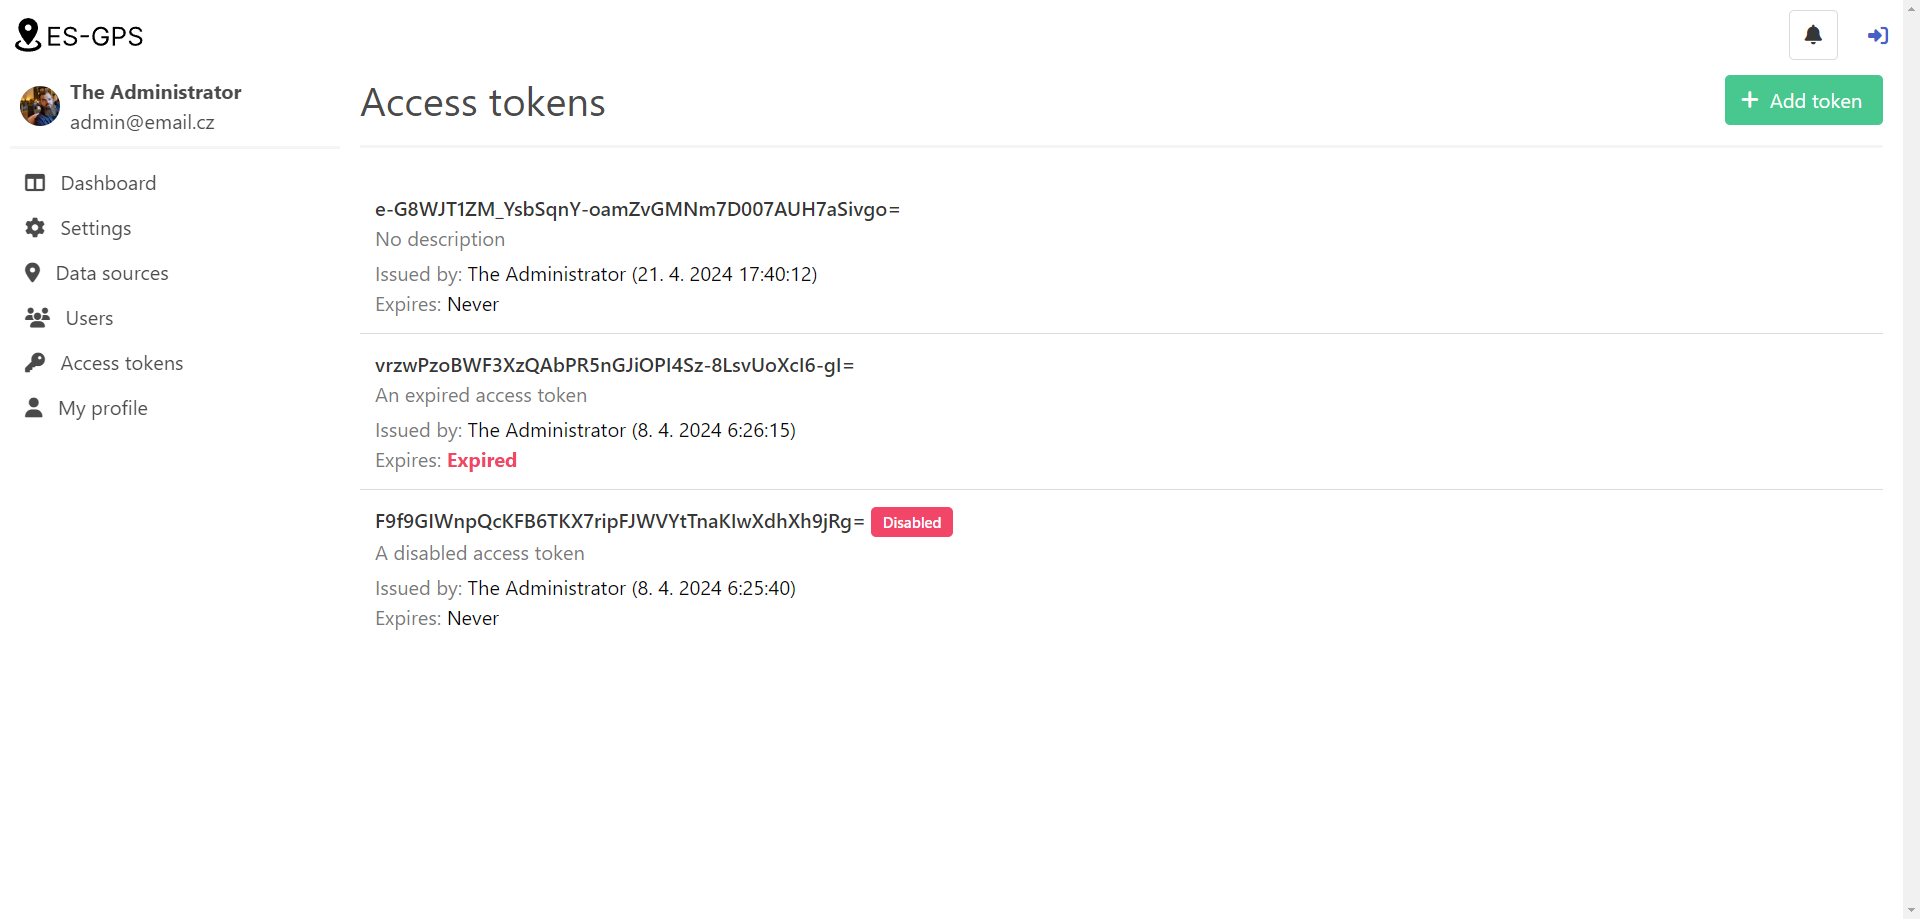
\includegraphics[width=1.2\textwidth]{appendix/tokens.png}}}
    \caption{The access token system}
\end{figure}

\section{Collected data}
\begin{figure}[H]
    \centering
	\makebox[\textwidth][c]{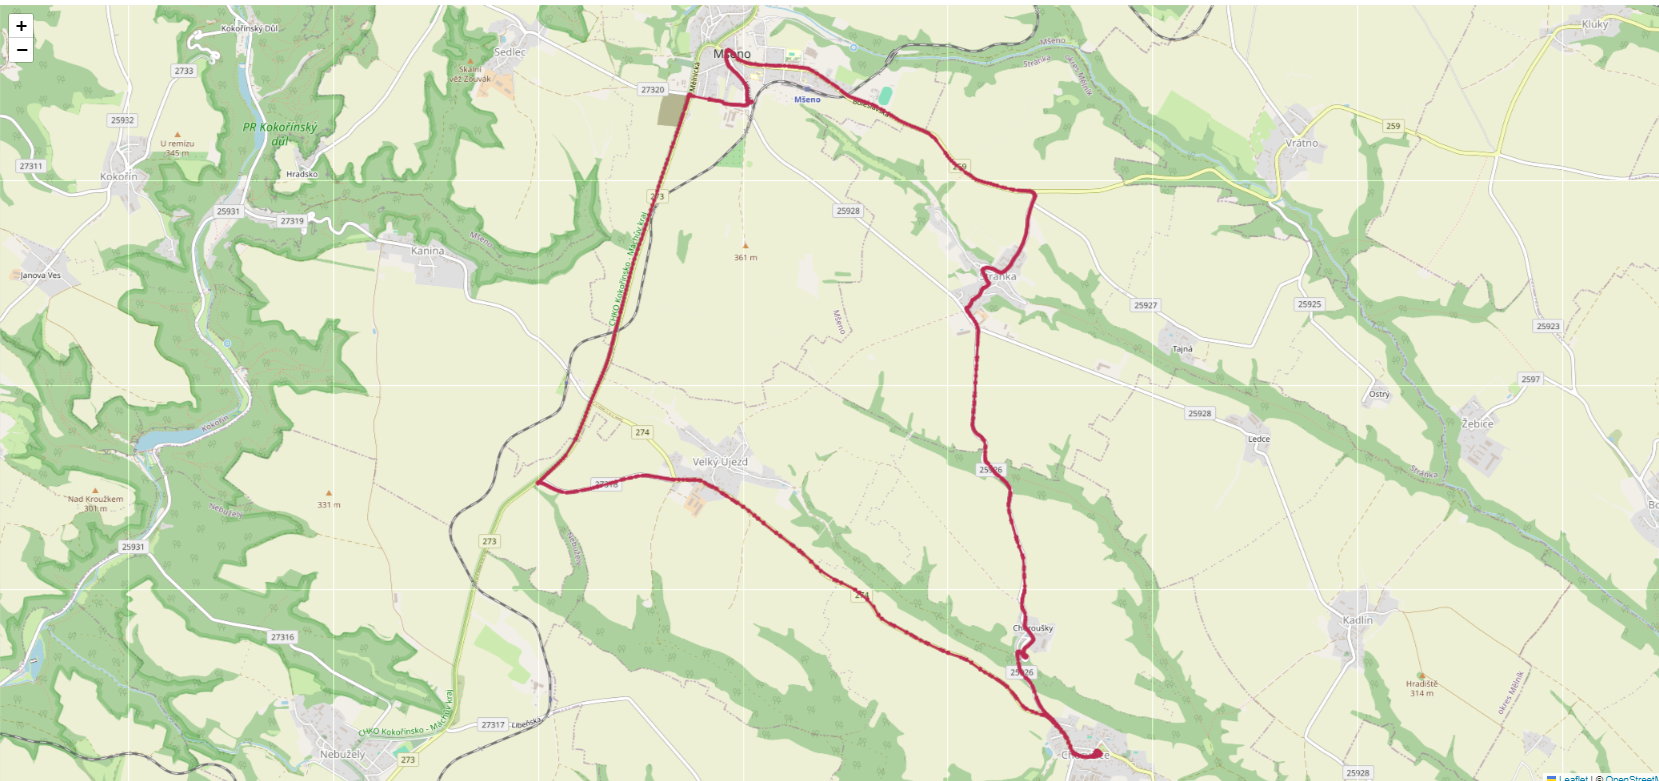
\includegraphics[width=1.2\textwidth]{appendix/okruh.png}}
    \caption{The testing lap (Mšeno - Stránka - Chorušice - Velký Újezd)}
    \label{fig:test-lap}
\end{figure}

\begin{figure}[H]
    \centering
	\makebox[\textwidth][c]{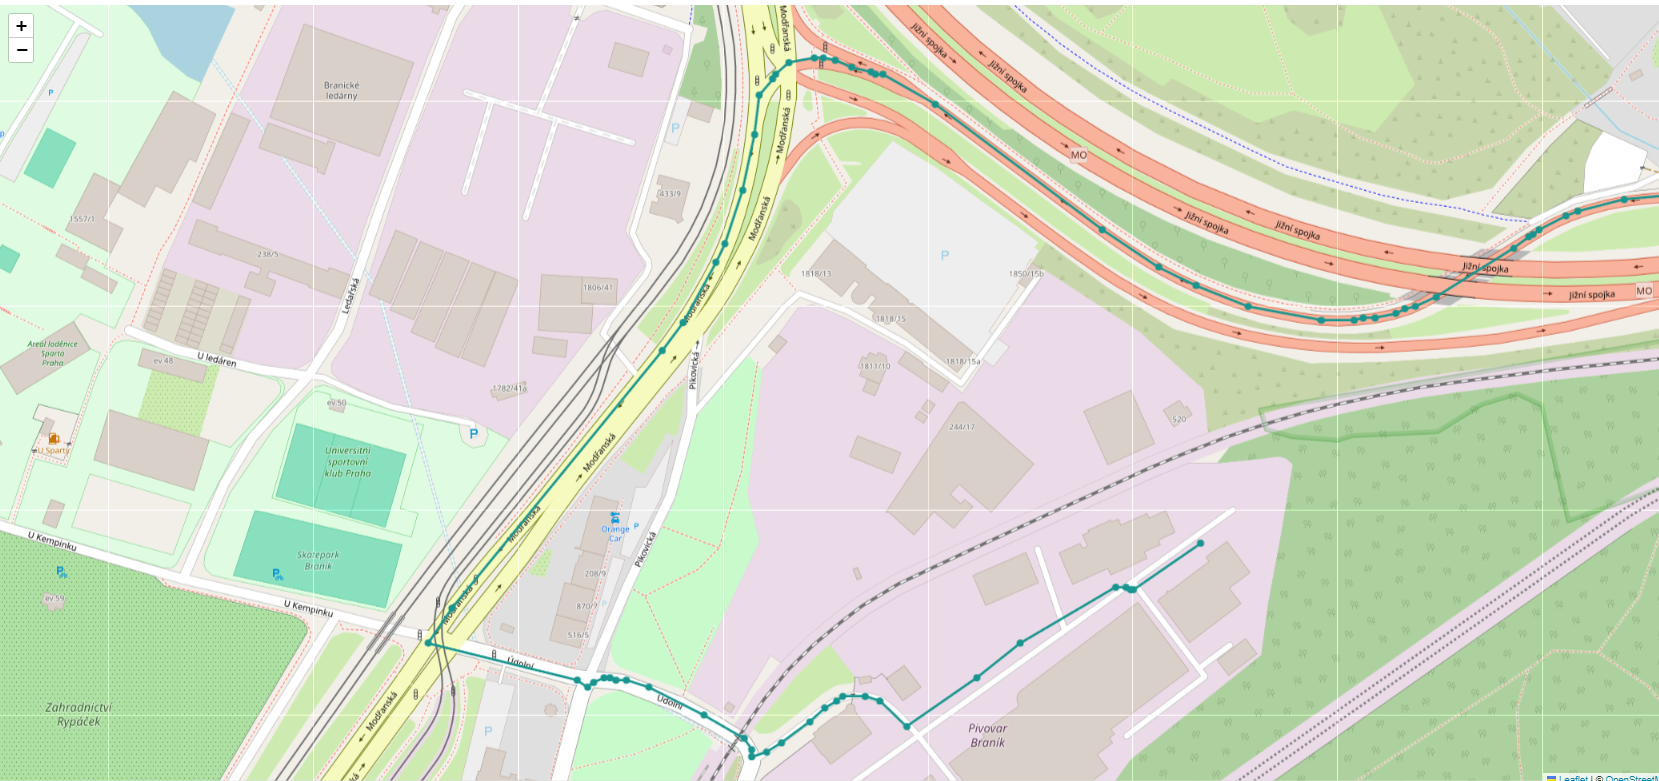
\includegraphics[width=1.2\textwidth]{appendix/xertec.png}}
     \caption{A Google Maps exported route (the theoretical perfect tracking outcome)}
    \label{fig:google-maps-export}
\end{figure}

\begin{figure}[H]
    \centering
	\makebox[\textwidth][c]{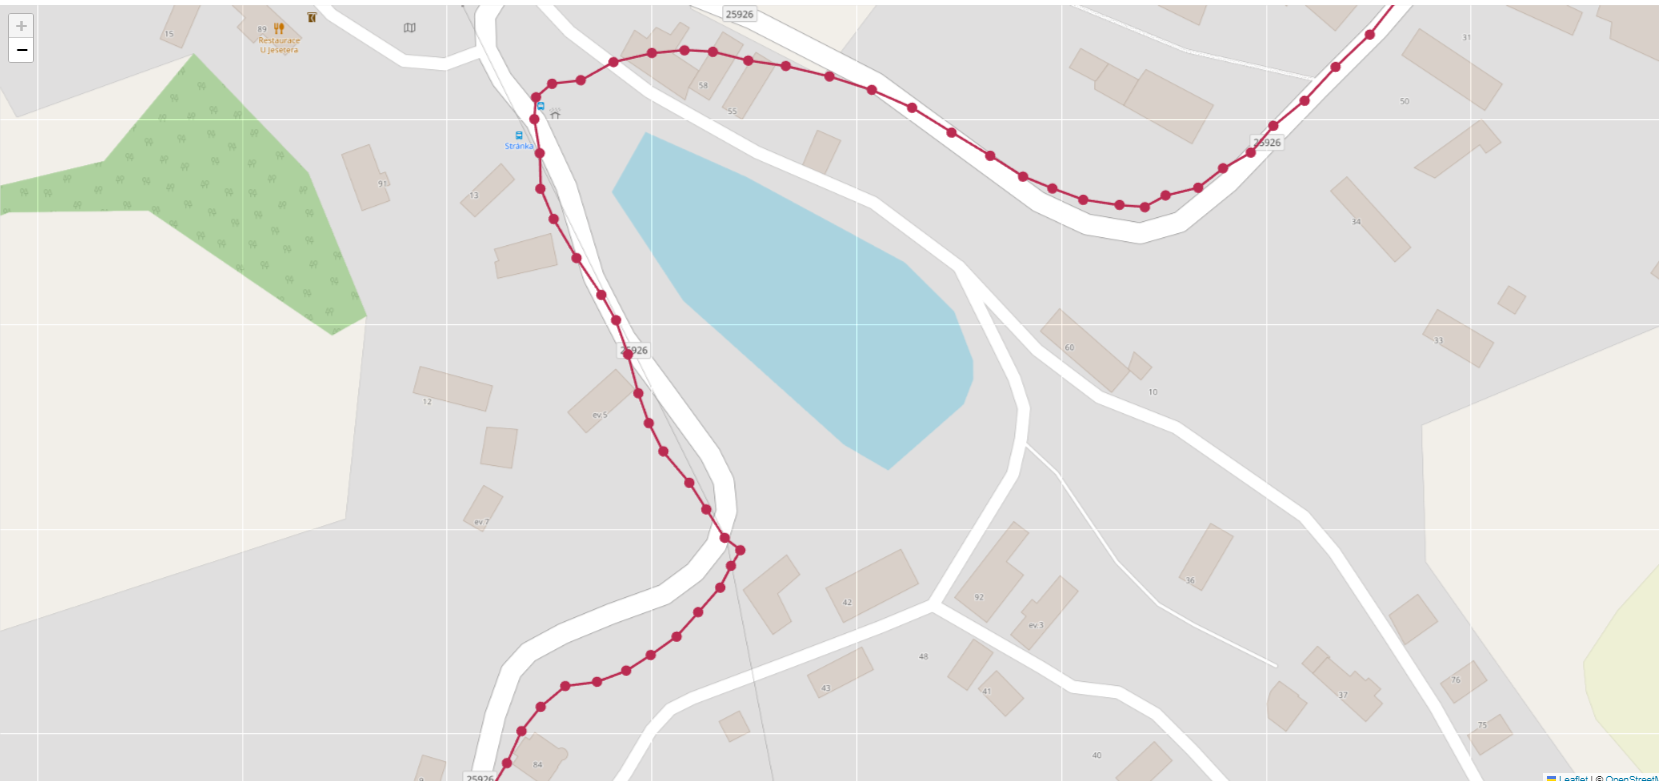
\includegraphics[width=1.2\textwidth]{appendix/1s-samplerate.png}}
    \caption{The amount of captured detail with a sampling rate of \textbf{1s}}
    \label{fig:1s-samplerate}
\end{figure}

\begin{figure}[H]
    \centering
	\makebox[\textwidth][c]{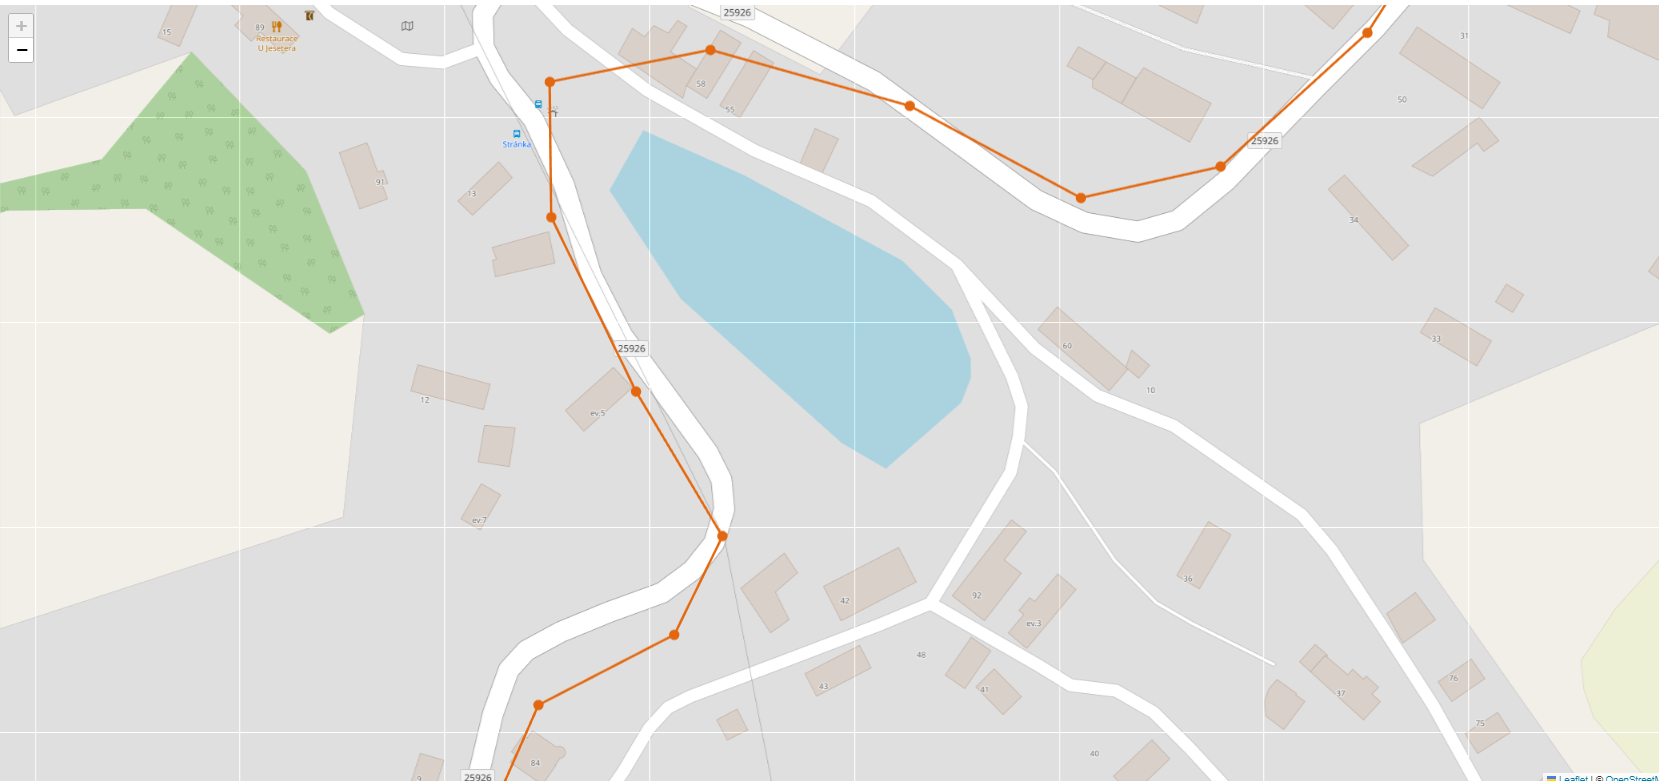
\includegraphics[width=1.2\textwidth]{appendix/5s-samplerate.png}}
     \caption{The amount of captured detail with a sampling rate of \textbf{5s}}
    \label{fig:5s-samplerate}
\end{figure}

\newpage

\section{Photos}

\begin{figure}[H]
    \centering
	\makebox[\textwidth][c]{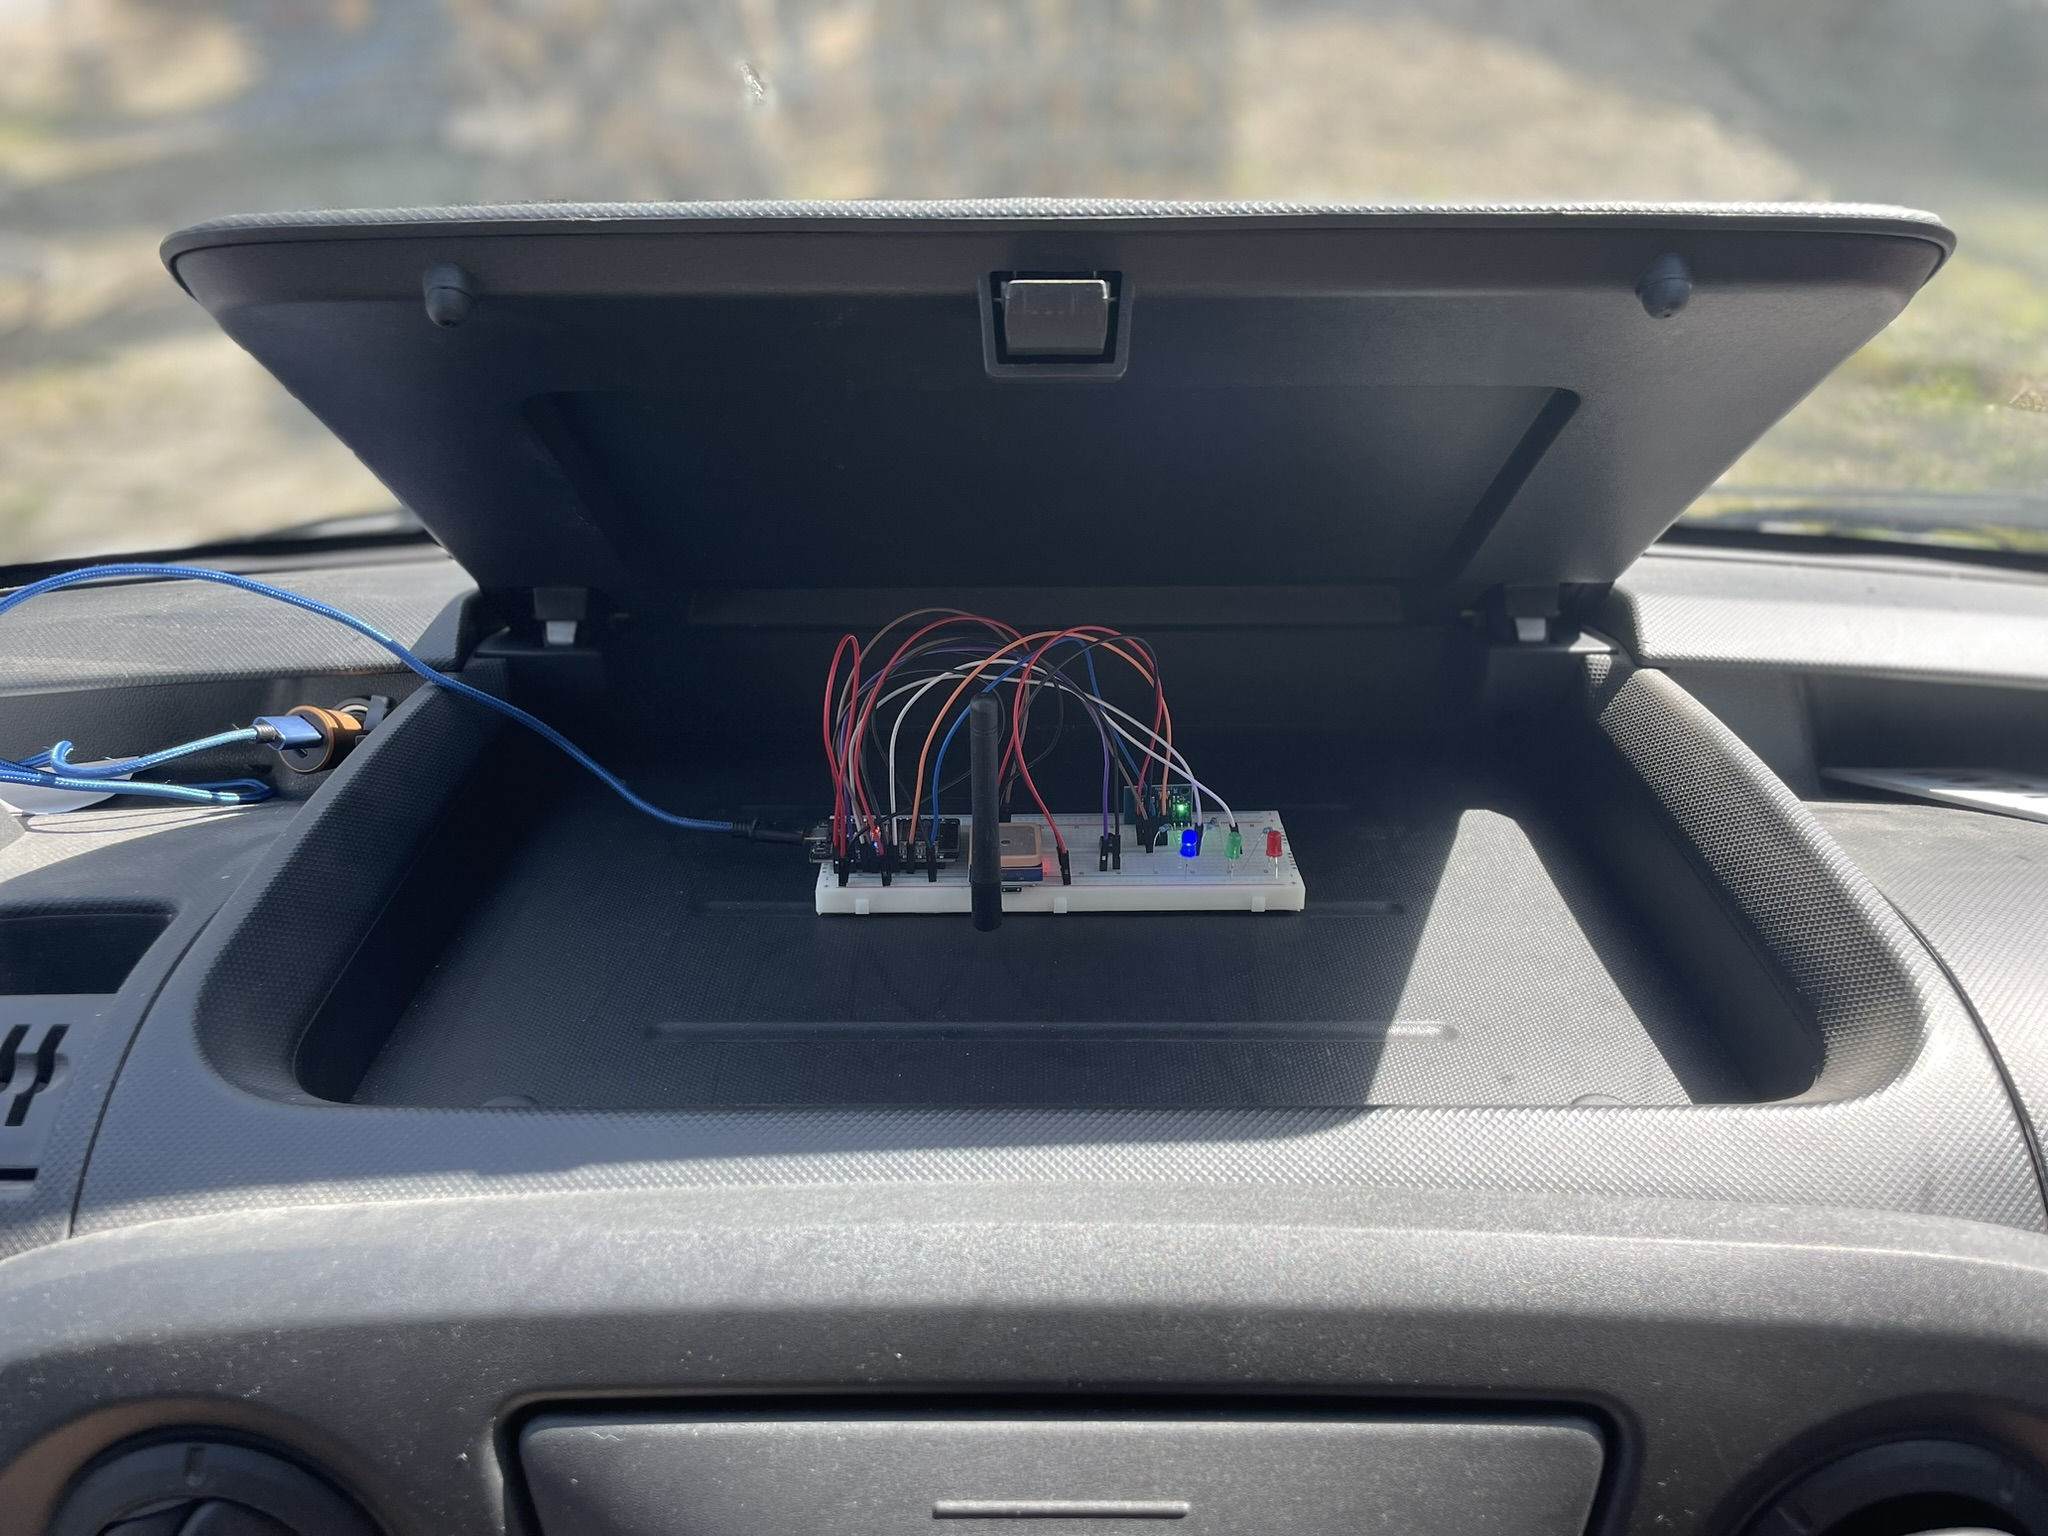
\includegraphics[width=1.2\textwidth]{appendix/car_deployment.JPEG}}
    \caption{The physical deployment of the hardware solution}
    \label{fig:physical-incar-deployment}
\end{figure}

\section{Miscellaneous}
A technical documentation for this project was conveniently compiled as part of the requirements for another class and published through GitHub Pages at \href{https://pzdrs.github.io/BP-docs/}{https://pzdrs.github.io/BP-docs/}.

\vspace*{\fill}

For linguistic and research purposes, the use of artificial intelligence was leveraged throughout some parts of the thesis, more specifically the \textit{ChatGPT 3.5}.
\end{document}